\documentclass[a4paper]{book}
\usepackage{makeidx}
\usepackage{graphicx}
\usepackage{multicol}
\usepackage{float}
\usepackage{listings}
\usepackage{color}
\usepackage{textcomp}
\usepackage{alltt}
\usepackage{times}
\usepackage{ifpdf}
\ifpdf
\usepackage[pdftex,
            pagebackref=true,
            colorlinks=true,
            linkcolor=blue,
            unicode
           ]{hyperref}
\else
\usepackage[ps2pdf,
            pagebackref=true,
            colorlinks=true,
            linkcolor=blue,
            unicode
           ]{hyperref}
\usepackage{pspicture}
\fi
\usepackage[utf8]{inputenc}
\usepackage{doxygen}
\lstset{language=C++,inputencoding=utf8,basicstyle=\footnotesize,breaklines=true,breakatwhitespace=true,tabsize=8,numbers=left }
\usepackage{YES}
\makeindex
\setcounter{tocdepth}{3}
\renewcommand{\footrulewidth}{0.4pt}
\begin{document}
\hypersetup{pageanchor=false}
\begin{titlepage}
\vspace*{7cm}
\begin{center}
{\Large Multistage software router energy saving scheme }\\
\vspace*{1cm}
{\large Generated by Doxygen 1.7.1}\\
\vspace*{0.5cm}
{\small Fri Mar 16 2012 15:20:11}\\
\end{center}
\end{titlepage}
\clearemptydoublepage
\pagenumbering{roman}
\tableofcontents
\clearemptydoublepage
\pagenumbering{arabic}
\hypersetup{pageanchor=true}
\chapter{Multistage software router energy saving scheme}
\label{index}\hypertarget{index}{}\hypertarget{index_intro}{}\section{Introduction}\label{index_intro}
An energy saving scheme for \href{multistage_software_router.pdf}{\tt {\bfseries multistage software router}}. 
\chapter{Class Index}
\section{Class Hierarchy}
This inheritance list is sorted roughly, but not completely, alphabetically:\begin{DoxyCompactList}
\item \contentsline{section}{device}{\pageref{classdevice}}{}
\begin{DoxyCompactList}
\item \contentsline{section}{multistage}{\pageref{classmultistage}}{}
\item \contentsline{section}{rLink}{\pageref{classrLink}}{}
\item \contentsline{section}{router}{\pageref{classrouter}}{}
\end{DoxyCompactList}
\item \contentsline{section}{graph}{\pageref{classgraph}}{}
\item \contentsline{section}{statistics}{\pageref{classstatistics}}{}
\item \contentsline{section}{timer}{\pageref{classtimer}}{}
\item \contentsline{section}{trafficgen}{\pageref{classtrafficgen}}{}
\end{DoxyCompactList}

\chapter{Class Index}
\section{Class List}
Here are the classes, structs, unions and interfaces with brief descriptions:\begin{DoxyCompactList}
\item\contentsline{section}{\hyperlink{classdevice}{device} (Basic class for devices in the multistage architecture )}{\pageref{classdevice}}{}
\item\contentsline{section}{\hyperlink{classgraph}{graph} (Graph class used for result display )}{\pageref{classgraph}}{}
\item\contentsline{section}{\hyperlink{classmultistage}{multistage} (Multistage architecture class reference )}{\pageref{classmultistage}}{}
\item\contentsline{section}{\hyperlink{classrLink}{rLink} (Router link class reference )}{\pageref{classrLink}}{}
\item\contentsline{section}{\hyperlink{classrouter}{router} (Multistage architecture router class reference )}{\pageref{classrouter}}{}
\item\contentsline{section}{\hyperlink{classstatistics}{statistics} (Statistics class to collect device states )}{\pageref{classstatistics}}{}
\item\contentsline{section}{\hyperlink{classtimer}{timer} (Basic class to calculate time difference )}{\pageref{classtimer}}{}
\item\contentsline{section}{\hyperlink{classtrafficgen}{trafficgen} (Traffic generator )}{\pageref{classtrafficgen}}{}
\end{DoxyCompactList}

\chapter{File Index}
\section{File List}
Here is a list of all files with brief descriptions:\begin{DoxyCompactList}
\item\contentsline{section}{/home/fikru/Desktop/fikru/research/code/online\_\-energy\_\-saving\_\-splittable/\hyperlink{bin__packing_8cpp}{bin\_\-packing.cpp} }{\pageref{bin__packing_8cpp}}{}
\item\contentsline{section}{/home/fikru/Desktop/fikru/research/code/online\_\-energy\_\-saving\_\-splittable/\hyperlink{configuration_8cpp}{configuration.cpp} }{\pageref{configuration_8cpp}}{}
\item\contentsline{section}{/home/fikru/Desktop/fikru/research/code/online\_\-energy\_\-saving\_\-splittable/\hyperlink{device_8cpp}{device.cpp} }{\pageref{device_8cpp}}{}
\item\contentsline{section}{/home/fikru/Desktop/fikru/research/code/online\_\-energy\_\-saving\_\-splittable/\hyperlink{display_8cpp}{display.cpp} }{\pageref{display_8cpp}}{}
\item\contentsline{section}{/home/fikru/Desktop/fikru/research/code/online\_\-energy\_\-saving\_\-splittable/\hyperlink{graph_8cpp}{graph.cpp} }{\pageref{graph_8cpp}}{}
\item\contentsline{section}{/home/fikru/Desktop/fikru/research/code/online\_\-energy\_\-saving\_\-splittable/\hyperlink{multistage_8cpp}{multistage.cpp} }{\pageref{multistage_8cpp}}{}
\item\contentsline{section}{/home/fikru/Desktop/fikru/research/code/online\_\-energy\_\-saving\_\-splittable/\hyperlink{rLink_8cpp}{rLink.cpp} }{\pageref{rLink_8cpp}}{}
\item\contentsline{section}{/home/fikru/Desktop/fikru/research/code/online\_\-energy\_\-saving\_\-splittable/\hyperlink{router_8cpp}{router.cpp} }{\pageref{router_8cpp}}{}
\item\contentsline{section}{/home/fikru/Desktop/fikru/research/code/online\_\-energy\_\-saving\_\-splittable/\hyperlink{SCESApplication_8cpp}{SCESApplication.cpp} }{\pageref{SCESApplication_8cpp}}{}
\item\contentsline{section}{/home/fikru/Desktop/fikru/research/code/online\_\-energy\_\-saving\_\-splittable/\hyperlink{sorter_8cpp}{sorter.cpp} }{\pageref{sorter_8cpp}}{}
\item\contentsline{section}{/home/fikru/Desktop/fikru/research/code/online\_\-energy\_\-saving\_\-splittable/\hyperlink{statistics_8cpp}{statistics.cpp} }{\pageref{statistics_8cpp}}{}
\item\contentsline{section}{/home/fikru/Desktop/fikru/research/code/online\_\-energy\_\-saving\_\-splittable/\hyperlink{timer_8cpp}{timer.cpp} }{\pageref{timer_8cpp}}{}
\item\contentsline{section}{/home/fikru/Desktop/fikru/research/code/online\_\-energy\_\-saving\_\-splittable/\hyperlink{trafficgen_8cpp}{trafficgen.cpp} }{\pageref{trafficgen_8cpp}}{}
\item\contentsline{section}{/home/fikru/Desktop/fikru/research/code/online\_\-energy\_\-saving\_\-splittable/include/\hyperlink{device_8h}{device.h} }{\pageref{device_8h}}{}
\item\contentsline{section}{/home/fikru/Desktop/fikru/research/code/online\_\-energy\_\-saving\_\-splittable/include/\hyperlink{global_8h}{global.h} }{\pageref{global_8h}}{}
\item\contentsline{section}{/home/fikru/Desktop/fikru/research/code/online\_\-energy\_\-saving\_\-splittable/include/\hyperlink{graph_8h}{graph.h} }{\pageref{graph_8h}}{}
\item\contentsline{section}{/home/fikru/Desktop/fikru/research/code/online\_\-energy\_\-saving\_\-splittable/include/\hyperlink{multistage_8h}{multistage.h} }{\pageref{multistage_8h}}{}
\item\contentsline{section}{/home/fikru/Desktop/fikru/research/code/online\_\-energy\_\-saving\_\-splittable/include/\hyperlink{rLink_8h}{rLink.h} }{\pageref{rLink_8h}}{}
\item\contentsline{section}{/home/fikru/Desktop/fikru/research/code/online\_\-energy\_\-saving\_\-splittable/include/\hyperlink{router_8h}{router.h} }{\pageref{router_8h}}{}
\item\contentsline{section}{/home/fikru/Desktop/fikru/research/code/online\_\-energy\_\-saving\_\-splittable/include/\hyperlink{statistics_8h}{statistics.h} }{\pageref{statistics_8h}}{}
\item\contentsline{section}{/home/fikru/Desktop/fikru/research/code/online\_\-energy\_\-saving\_\-splittable/include/\hyperlink{timer_8h}{timer.h} }{\pageref{timer_8h}}{}
\item\contentsline{section}{/home/fikru/Desktop/fikru/research/code/online\_\-energy\_\-saving\_\-splittable/include/\hyperlink{trafficgen_8h}{trafficgen.h} }{\pageref{trafficgen_8h}}{}
\end{DoxyCompactList}

\chapter{Class Documentation}
\hypertarget{classdevice}{
\section{device Class Reference}
\label{classdevice}\index{device@{device}}
}


Basic class for devices in the multistage architecture.  




{\ttfamily \#include $<$device.h$>$}

Inheritance diagram for device:\begin{figure}[H]
\begin{center}
\leavevmode
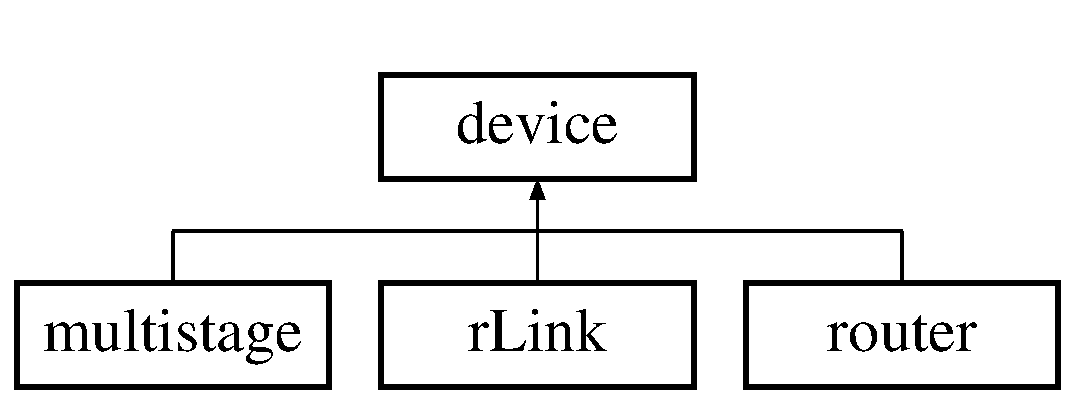
\includegraphics[height=2.000000cm]{classdevice}
\end{center}
\end{figure}
\subsection*{Public Member Functions}
\begin{DoxyCompactItemize}
\item 
\hyperlink{classdevice_a95ab42e0b2e738637d3414347fa5559c}{device} ()
\begin{DoxyCompactList}\small\item\em Construct multistage architecture and routers there in. \item\end{DoxyCompactList}\item 
\hyperlink{classdevice_a57b9c4ac7a8bd970b81b1154ae79a5de}{device} (int, string, double, double, int, int)
\item 
\hyperlink{classdevice_a3aa4a2a68f49628354dbe33de584f726}{device} (int, string, double, double, int)
\begin{DoxyCompactList}\small\item\em Construct multistage architecture and routers there in. \item\end{DoxyCompactList}\item 
\hyperlink{classdevice_a08545ac77231c68a27c32633a9730a33}{$\sim$device} ()
\begin{DoxyCompactList}\small\item\em destructor \item\end{DoxyCompactList}\item 
int \hyperlink{classdevice_a5b73405bc8184085f92306d4f323b572}{getID} ()
\begin{DoxyCompactList}\small\item\em Gets device identification number. \item\end{DoxyCompactList}\item 
string \hyperlink{classdevice_a9dc7119476febd7ba47060d74ba37e20}{getName} ()
\begin{DoxyCompactList}\small\item\em Gets device name. \item\end{DoxyCompactList}\item 
double \hyperlink{classdevice_ae444f5ce9e539235bc5df36f7b47609c}{getCapacity} ()
\begin{DoxyCompactList}\small\item\em Gets device capacity. \item\end{DoxyCompactList}\item 
double \hyperlink{classdevice_af7b6d78ad457ad75a5f3ed2b40266017}{getPower} ()
\begin{DoxyCompactList}\small\item\em Gets device power consumption. \item\end{DoxyCompactList}\item 
bool \hyperlink{classdevice_a287ef719b436c552cb78f498869ce590}{getState} ()
\begin{DoxyCompactList}\small\item\em Gets device state. \item\end{DoxyCompactList}\item 
int \hyperlink{classdevice_aba1387d01eac1fa58a5386395b368384}{getNr\_\-device} ()
\begin{DoxyCompactList}\small\item\em Gets number of devices contained inside a device. \item\end{DoxyCompactList}\item 
void \hyperlink{classdevice_a66b66e2bce25b091d651ee6336f6f40e}{setCapacity} (double)
\begin{DoxyCompactList}\small\item\em Sets device capacity. \item\end{DoxyCompactList}\item 
void \hyperlink{classdevice_a43b8093ad785d5b5787751a7ede0ae73}{setPower} (double)
\begin{DoxyCompactList}\small\item\em Sets device power consumption. \item\end{DoxyCompactList}\item 
void \hyperlink{classdevice_a8479767364d2d7a6e349552eb6bae023}{setState} (bool)
\begin{DoxyCompactList}\small\item\em Sets device state. \item\end{DoxyCompactList}\end{DoxyCompactItemize}


\subsection{Detailed Description}
Basic class for devices in the multistage architecture. Inherited by multistage, routers and links 

\subsection{Constructor \& Destructor Documentation}
\hypertarget{classdevice_a95ab42e0b2e738637d3414347fa5559c}{
\index{device@{device}!device@{device}}
\index{device@{device}!device@{device}}
\subsubsection[{device}]{\setlength{\rightskip}{0pt plus 5cm}device::device (
\begin{DoxyParamCaption}
{}
\end{DoxyParamCaption}
)\hspace{0.3cm}{\ttfamily  \mbox{[}inline\mbox{]}}}}
\label{classdevice_a95ab42e0b2e738637d3414347fa5559c}


Construct multistage architecture and routers there in. 


\begin{DoxyParams}{Parameters}
\item[{\em ID}]device identification number \item[{\em name}]device name \item[{\em capacity}]device capacity \item[{\em power}]device power consumption \item[{\em nr\_\-device}]number of devices contained inside: multistage contain routers and routers contain links \item[{\em state}]device state: ON/OFF \end{DoxyParams}
\hypertarget{classdevice_a57b9c4ac7a8bd970b81b1154ae79a5de}{
\index{device@{device}!device@{device}}
\index{device@{device}!device@{device}}
\subsubsection[{device}]{\setlength{\rightskip}{0pt plus 5cm}device::device (
\begin{DoxyParamCaption}
\item[{int}]{ ID, }
\item[{string}]{ name, }
\item[{double}]{ capacity, }
\item[{double}]{ power, }
\item[{int}]{ state, }
\item[{int}]{ nr\_\-device}
\end{DoxyParamCaption}
)}}
\label{classdevice_a57b9c4ac7a8bd970b81b1154ae79a5de}
\hypertarget{classdevice_a3aa4a2a68f49628354dbe33de584f726}{
\index{device@{device}!device@{device}}
\index{device@{device}!device@{device}}
\subsubsection[{device}]{\setlength{\rightskip}{0pt plus 5cm}device::device (
\begin{DoxyParamCaption}
\item[{int}]{ ID, }
\item[{string}]{ name, }
\item[{double}]{ capacity, }
\item[{double}]{ power, }
\item[{int}]{ state}
\end{DoxyParamCaption}
)}}
\label{classdevice_a3aa4a2a68f49628354dbe33de584f726}


Construct multistage architecture and routers there in. 


\begin{DoxyParams}{Parameters}
\item[{\em ID}]device identification \item[{\em name}]device name \item[{\em capacity}]device capacity \item[{\em power}]device power consumption \item[{\em state}]device state: ON/OFF \end{DoxyParams}
\hypertarget{classdevice_a08545ac77231c68a27c32633a9730a33}{
\index{device@{device}!$\sim$device@{$\sim$device}}
\index{$\sim$device@{$\sim$device}!device@{device}}
\subsubsection[{$\sim$device}]{\setlength{\rightskip}{0pt plus 5cm}device::$\sim$device (
\begin{DoxyParamCaption}
{}
\end{DoxyParamCaption}
)\hspace{0.3cm}{\ttfamily  \mbox{[}inline\mbox{]}}}}
\label{classdevice_a08545ac77231c68a27c32633a9730a33}


destructor 



\subsection{Member Function Documentation}
\hypertarget{classdevice_ae444f5ce9e539235bc5df36f7b47609c}{
\index{device@{device}!getCapacity@{getCapacity}}
\index{getCapacity@{getCapacity}!device@{device}}
\subsubsection[{getCapacity}]{\setlength{\rightskip}{0pt plus 5cm}double device::getCapacity (
\begin{DoxyParamCaption}
{}
\end{DoxyParamCaption}
)}}
\label{classdevice_ae444f5ce9e539235bc5df36f7b47609c}


Gets device capacity. 

\begin{DoxyReturn}{Returns}
device capacity 
\end{DoxyReturn}
\hypertarget{classdevice_a5b73405bc8184085f92306d4f323b572}{
\index{device@{device}!getID@{getID}}
\index{getID@{getID}!device@{device}}
\subsubsection[{getID}]{\setlength{\rightskip}{0pt plus 5cm}int device::getID (
\begin{DoxyParamCaption}
{}
\end{DoxyParamCaption}
)}}
\label{classdevice_a5b73405bc8184085f92306d4f323b572}


Gets device identification number. 

\begin{DoxyReturn}{Returns}
device identification number 
\end{DoxyReturn}
\hypertarget{classdevice_a9dc7119476febd7ba47060d74ba37e20}{
\index{device@{device}!getName@{getName}}
\index{getName@{getName}!device@{device}}
\subsubsection[{getName}]{\setlength{\rightskip}{0pt plus 5cm}string device::getName (
\begin{DoxyParamCaption}
{}
\end{DoxyParamCaption}
)}}
\label{classdevice_a9dc7119476febd7ba47060d74ba37e20}


Gets device name. 

\begin{DoxyReturn}{Returns}
device name 
\end{DoxyReturn}
\hypertarget{classdevice_aba1387d01eac1fa58a5386395b368384}{
\index{device@{device}!getNr\_\-device@{getNr\_\-device}}
\index{getNr\_\-device@{getNr\_\-device}!device@{device}}
\subsubsection[{getNr\_\-device}]{\setlength{\rightskip}{0pt plus 5cm}int device::getNr\_\-device (
\begin{DoxyParamCaption}
{}
\end{DoxyParamCaption}
)}}
\label{classdevice_aba1387d01eac1fa58a5386395b368384}


Gets number of devices contained inside a device. 

\begin{DoxyReturn}{Returns}
Number of devices contained inside a device. For example the number of routers in a multistage architecture 
\end{DoxyReturn}
\hypertarget{classdevice_af7b6d78ad457ad75a5f3ed2b40266017}{
\index{device@{device}!getPower@{getPower}}
\index{getPower@{getPower}!device@{device}}
\subsubsection[{getPower}]{\setlength{\rightskip}{0pt plus 5cm}double device::getPower (
\begin{DoxyParamCaption}
{}
\end{DoxyParamCaption}
)}}
\label{classdevice_af7b6d78ad457ad75a5f3ed2b40266017}


Gets device power consumption. 

\begin{DoxyReturn}{Returns}
device power 
\end{DoxyReturn}
\hypertarget{classdevice_a287ef719b436c552cb78f498869ce590}{
\index{device@{device}!getState@{getState}}
\index{getState@{getState}!device@{device}}
\subsubsection[{getState}]{\setlength{\rightskip}{0pt plus 5cm}bool device::getState (
\begin{DoxyParamCaption}
{}
\end{DoxyParamCaption}
)}}
\label{classdevice_a287ef719b436c552cb78f498869ce590}


Gets device state. 

\begin{DoxyReturn}{Returns}
device state 
\end{DoxyReturn}
\hypertarget{classdevice_a66b66e2bce25b091d651ee6336f6f40e}{
\index{device@{device}!setCapacity@{setCapacity}}
\index{setCapacity@{setCapacity}!device@{device}}
\subsubsection[{setCapacity}]{\setlength{\rightskip}{0pt plus 5cm}void device::setCapacity (
\begin{DoxyParamCaption}
\item[{double}]{ capacity}
\end{DoxyParamCaption}
)}}
\label{classdevice_a66b66e2bce25b091d651ee6336f6f40e}


Sets device capacity. 


\begin{DoxyParams}{Parameters}
\item[{\em capacity}]capacity of the device \end{DoxyParams}
\hypertarget{classdevice_a43b8093ad785d5b5787751a7ede0ae73}{
\index{device@{device}!setPower@{setPower}}
\index{setPower@{setPower}!device@{device}}
\subsubsection[{setPower}]{\setlength{\rightskip}{0pt plus 5cm}void device::setPower (
\begin{DoxyParamCaption}
\item[{double}]{ power}
\end{DoxyParamCaption}
)}}
\label{classdevice_a43b8093ad785d5b5787751a7ede0ae73}


Sets device power consumption. 


\begin{DoxyParams}{Parameters}
\item[{\em power}]power consumption of the device \end{DoxyParams}
\hypertarget{classdevice_a8479767364d2d7a6e349552eb6bae023}{
\index{device@{device}!setState@{setState}}
\index{setState@{setState}!device@{device}}
\subsubsection[{setState}]{\setlength{\rightskip}{0pt plus 5cm}void device::setState (
\begin{DoxyParamCaption}
\item[{bool}]{ state}
\end{DoxyParamCaption}
)}}
\label{classdevice_a8479767364d2d7a6e349552eb6bae023}


Sets device state. 


\begin{DoxyParams}{Parameters}
\item[{\em state}]the stare fo the device: ON/OFF \end{DoxyParams}


The documentation for this class was generated from the following files:\begin{DoxyCompactItemize}
\item 
/home/fikru/Desktop/fikru/research/code/online\_\-energy\_\-saving\_\-splittable/include/\hyperlink{device_8h}{device.h}\item 
/home/fikru/Desktop/fikru/research/code/online\_\-energy\_\-saving\_\-splittable/\hyperlink{device_8cpp}{device.cpp}\end{DoxyCompactItemize}

\hypertarget{classgraph}{
\section{graph Class Reference}
\label{classgraph}\index{graph@{graph}}
}


Graph class used for result display.  




{\ttfamily \#include $<$graph.h$>$}

\subsection*{Public Member Functions}
\begin{DoxyCompactItemize}
\item 
\hyperlink{classgraph_a6aaa56b4528d2fdb8f0ecd97e04f6651}{graph} ()
\begin{DoxyCompactList}\small\item\em constructor \item\end{DoxyCompactList}\item 
\hyperlink{classgraph_aeb62eaf197cdcb4800fa016eebc3d55a}{$\sim$graph} ()
\begin{DoxyCompactList}\small\item\em destructor \item\end{DoxyCompactList}\item 
vector$<$ float $>$ \hyperlink{classgraph_ab3640a345a45d78395b84a314cfaa6e9}{getLoad} ()
\begin{DoxyCompactList}\small\item\em gets list of traffic load \item\end{DoxyCompactList}\item 
vector$<$ double $>$ \hyperlink{classgraph_af576a52d2b39a3126dbf6cf56011a3ae}{getPower} ()
\begin{DoxyCompactList}\small\item\em gets list of architecture power consumption corresponding to each load \item\end{DoxyCompactList}\item 
void \hyperlink{classgraph_af551af99376a1d3fa4e0181a682aa224}{setLoad} (float)
\begin{DoxyCompactList}\small\item\em sets traffic load \item\end{DoxyCompactList}\item 
void \hyperlink{classgraph_ac78fb63912db679ad11b55dd25021145}{setpower} (double)
\begin{DoxyCompactList}\small\item\em set current objective \item\end{DoxyCompactList}\end{DoxyCompactItemize}


\subsection{Detailed Description}
Graph class used for result display. 

\subsection{Constructor \& Destructor Documentation}
\hypertarget{classgraph_a6aaa56b4528d2fdb8f0ecd97e04f6651}{
\index{graph@{graph}!graph@{graph}}
\index{graph@{graph}!graph@{graph}}
\subsubsection[{graph}]{\setlength{\rightskip}{0pt plus 5cm}graph::graph (
\begin{DoxyParamCaption}
{}
\end{DoxyParamCaption}
)}}
\label{classgraph_a6aaa56b4528d2fdb8f0ecd97e04f6651}


constructor 

\hypertarget{classgraph_aeb62eaf197cdcb4800fa016eebc3d55a}{
\index{graph@{graph}!$\sim$graph@{$\sim$graph}}
\index{$\sim$graph@{$\sim$graph}!graph@{graph}}
\subsubsection[{$\sim$graph}]{\setlength{\rightskip}{0pt plus 5cm}graph::$\sim$graph (
\begin{DoxyParamCaption}
{}
\end{DoxyParamCaption}
)\hspace{0.3cm}{\ttfamily  \mbox{[}inline\mbox{]}}}}
\label{classgraph_aeb62eaf197cdcb4800fa016eebc3d55a}


destructor 



\subsection{Member Function Documentation}
\hypertarget{classgraph_ab3640a345a45d78395b84a314cfaa6e9}{
\index{graph@{graph}!getLoad@{getLoad}}
\index{getLoad@{getLoad}!graph@{graph}}
\subsubsection[{getLoad}]{\setlength{\rightskip}{0pt plus 5cm}vector$<$ float $>$ graph::getLoad (
\begin{DoxyParamCaption}
{}
\end{DoxyParamCaption}
)}}
\label{classgraph_ab3640a345a45d78395b84a314cfaa6e9}


gets list of traffic load 

\hypertarget{classgraph_af576a52d2b39a3126dbf6cf56011a3ae}{
\index{graph@{graph}!getPower@{getPower}}
\index{getPower@{getPower}!graph@{graph}}
\subsubsection[{getPower}]{\setlength{\rightskip}{0pt plus 5cm}vector$<$ double $>$ graph::getPower (
\begin{DoxyParamCaption}
{}
\end{DoxyParamCaption}
)}}
\label{classgraph_af576a52d2b39a3126dbf6cf56011a3ae}


gets list of architecture power consumption corresponding to each load 

\hypertarget{classgraph_af551af99376a1d3fa4e0181a682aa224}{
\index{graph@{graph}!setLoad@{setLoad}}
\index{setLoad@{setLoad}!graph@{graph}}
\subsubsection[{setLoad}]{\setlength{\rightskip}{0pt plus 5cm}void graph::setLoad (
\begin{DoxyParamCaption}
\item[{float}]{ load}
\end{DoxyParamCaption}
)}}
\label{classgraph_af551af99376a1d3fa4e0181a682aa224}


sets traffic load 


\begin{DoxyParams}{Parameters}
\item[{\em load}]current traffic load \end{DoxyParams}
\hypertarget{classgraph_ac78fb63912db679ad11b55dd25021145}{
\index{graph@{graph}!setpower@{setpower}}
\index{setpower@{setpower}!graph@{graph}}
\subsubsection[{setpower}]{\setlength{\rightskip}{0pt plus 5cm}void graph::setpower (
\begin{DoxyParamCaption}
\item[{double}]{ power}
\end{DoxyParamCaption}
)}}
\label{classgraph_ac78fb63912db679ad11b55dd25021145}


set current objective 


\begin{DoxyParams}{Parameters}
\item[{\em power}]current power consumption of the architecture \end{DoxyParams}


The documentation for this class was generated from the following files:\begin{DoxyCompactItemize}
\item 
/home/fikru/Desktop/fikru/research/code/online\_\-energy\_\-saving\_\-splittable/include/\hyperlink{graph_8h}{graph.h}\item 
/home/fikru/Desktop/fikru/research/code/online\_\-energy\_\-saving\_\-splittable/\hyperlink{graph_8cpp}{graph.cpp}\end{DoxyCompactItemize}

\hypertarget{classmultistage}{
\section{multistage Class Reference}
\label{classmultistage}\index{multistage@{multistage}}
}


Multistage architecture class reference.  




{\ttfamily \#include $<$multistage.h$>$}

Inheritance diagram for multistage:\begin{figure}[H]
\begin{center}
\leavevmode
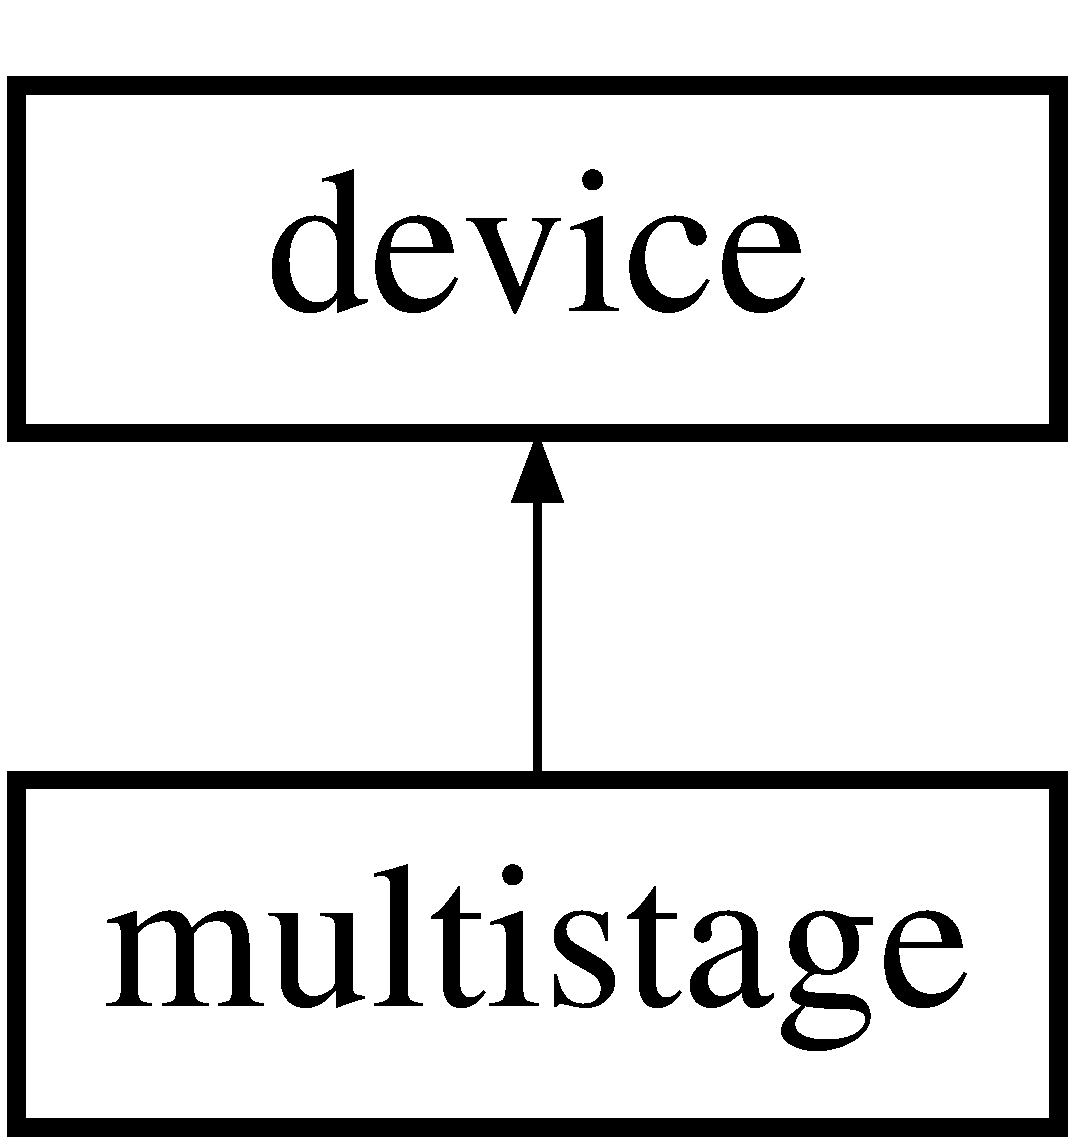
\includegraphics[height=2.000000cm]{classmultistage}
\end{center}
\end{figure}
\subsection*{Public Member Functions}
\begin{DoxyCompactItemize}
\item 
\hyperlink{classmultistage_adcbb45a38e0184f037cdc03504dced05}{multistage} (int, string, double, double, int, int)
\begin{DoxyCompactList}\small\item\em Construct a router. \item\end{DoxyCompactList}\item 
\hyperlink{classmultistage_a3ce104e1cd528efc9f4f2b8b8c2f54a7}{$\sim$multistage} ()
\begin{DoxyCompactList}\small\item\em Destructor. \item\end{DoxyCompactList}\item 
list$<$ \hyperlink{classrouter}{router} $>$ \hyperlink{classmultistage_ad42d7006ba661c60eb4958f8534ad89a}{getRList} ()
\begin{DoxyCompactList}\small\item\em Gets list of routers in an architecture. \item\end{DoxyCompactList}\item 
void \hyperlink{classmultistage_a6f79ee151acaff9a49e06a3300371a2c}{setRList} (\hyperlink{classrouter}{router})
\begin{DoxyCompactList}\small\item\em Sets an architecture's router list. \item\end{DoxyCompactList}\end{DoxyCompactItemize}


\subsection{Detailed Description}
Multistage architecture class reference. It inherits device class and creates a new multistage architecture with list of routers and sets total architecture actual capacity.

{\bfseries Usage Example:} 
\begin{DoxyCode}
 multistage *m = new multistage(1, "mssr", 0, 0, 0, 0)
\end{DoxyCode}
 \begin{DoxySeeAlso}{See also}
\hyperlink{classdevice_a57b9c4ac7a8bd970b81b1154ae79a5de}{device(int ,string ,double ,double ,int ,int )} 
\end{DoxySeeAlso}


\subsection{Constructor \& Destructor Documentation}
\hypertarget{classmultistage_adcbb45a38e0184f037cdc03504dced05}{
\index{multistage@{multistage}!multistage@{multistage}}
\index{multistage@{multistage}!multistage@{multistage}}
\subsubsection[{multistage}]{\setlength{\rightskip}{0pt plus 5cm}multistage::multistage (
\begin{DoxyParamCaption}
\item[{int}]{ ID, }
\item[{string}]{ name, }
\item[{double}]{ capacity, }
\item[{double}]{ power, }
\item[{int}]{ state, }
\item[{int}]{ nr\_\-routers}
\end{DoxyParamCaption}
)}}
\label{classmultistage_adcbb45a38e0184f037cdc03504dced05}


Construct a router. 


\begin{DoxyParams}{Parameters}
\item[{\em ID}]multistage architecture identification number \item[{\em name}]multistage architecture name \item[{\em capacity}]multistage architecture capacity \item[{\em power}]multistage architecture power consumption \item[{\em nr\_\-routers}]number of routers contained inside a multistage architecture \item[{\em state}]a multistage architecture state: ON/OFF \end{DoxyParams}
\begin{DoxySeeAlso}{See also}
\hyperlink{classdevice_a57b9c4ac7a8bd970b81b1154ae79a5de}{device(int ,string ,double ,double ,int ,int )} 
\end{DoxySeeAlso}
\hypertarget{classmultistage_a3ce104e1cd528efc9f4f2b8b8c2f54a7}{
\index{multistage@{multistage}!$\sim$multistage@{$\sim$multistage}}
\index{$\sim$multistage@{$\sim$multistage}!multistage@{multistage}}
\subsubsection[{$\sim$multistage}]{\setlength{\rightskip}{0pt plus 5cm}multistage::$\sim$multistage (
\begin{DoxyParamCaption}
{}
\end{DoxyParamCaption}
)\hspace{0.3cm}{\ttfamily  \mbox{[}inline\mbox{]}}}}
\label{classmultistage_a3ce104e1cd528efc9f4f2b8b8c2f54a7}


Destructor. 



\subsection{Member Function Documentation}
\hypertarget{classmultistage_ad42d7006ba661c60eb4958f8534ad89a}{
\index{multistage@{multistage}!getRList@{getRList}}
\index{getRList@{getRList}!multistage@{multistage}}
\subsubsection[{getRList}]{\setlength{\rightskip}{0pt plus 5cm}list$<$ {\bf router} $>$ multistage::getRList (
\begin{DoxyParamCaption}
{}
\end{DoxyParamCaption}
)}}
\label{classmultistage_ad42d7006ba661c60eb4958f8534ad89a}


Gets list of routers in an architecture. 

\begin{DoxyReturn}{Returns}
a multistage architecture's router list 
\end{DoxyReturn}
\hypertarget{classmultistage_a6f79ee151acaff9a49e06a3300371a2c}{
\index{multistage@{multistage}!setRList@{setRList}}
\index{setRList@{setRList}!multistage@{multistage}}
\subsubsection[{setRList}]{\setlength{\rightskip}{0pt plus 5cm}void multistage::setRList (
\begin{DoxyParamCaption}
\item[{{\bf router}}]{ r}
\end{DoxyParamCaption}
)}}
\label{classmultistage_a6f79ee151acaff9a49e06a3300371a2c}


Sets an architecture's router list. 


\begin{DoxyParams}{Parameters}
\item[{\em r}]router with all its attributes \end{DoxyParams}


The documentation for this class was generated from the following files:\begin{DoxyCompactItemize}
\item 
/home/fikru/Desktop/fikru/research/code/online\_\-energy\_\-saving\_\-splittable/include/\hyperlink{multistage_8h}{multistage.h}\item 
/home/fikru/Desktop/fikru/research/code/online\_\-energy\_\-saving\_\-splittable/\hyperlink{multistage_8cpp}{multistage.cpp}\end{DoxyCompactItemize}

\hypertarget{classrLink}{
\section{rLink Class Reference}
\label{classrLink}\index{rLink@{rLink}}
}


Router link class reference.  




{\ttfamily \#include $<$rLink.h$>$}

Inheritance diagram for rLink:\begin{figure}[H]
\begin{center}
\leavevmode
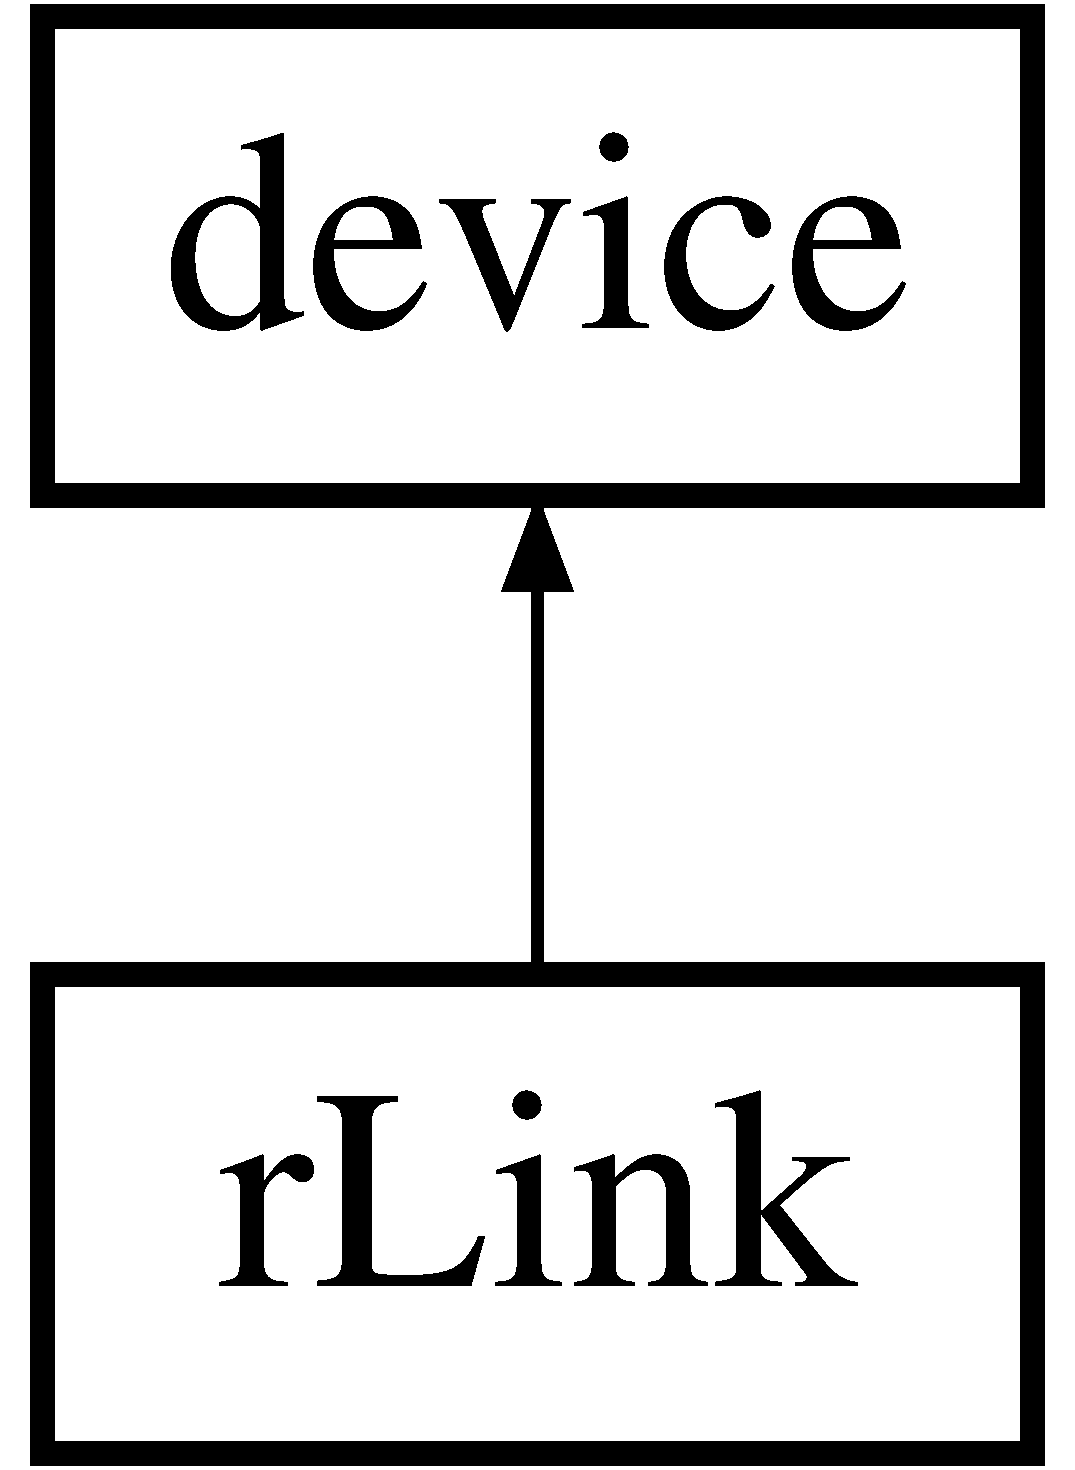
\includegraphics[height=2.000000cm]{classrLink}
\end{center}
\end{figure}
\subsection*{Public Member Functions}
\begin{DoxyCompactItemize}
\item 
\hyperlink{classrLink_acd7f5f66409693e86cd33e4a6e6964b8}{rLink} (int, string, double, double, int)
\begin{DoxyCompactList}\small\item\em Construct a link. \item\end{DoxyCompactList}\item 
\hyperlink{classrLink_ac2f6e30278ba2967b96086435711f672}{$\sim$rLink} ()
\begin{DoxyCompactList}\small\item\em Destructor. \item\end{DoxyCompactList}\item 
double \hyperlink{classrLink_aa840b5668425c224a451ec1663754a82}{getResidual} ()
\begin{DoxyCompactList}\small\item\em Gets residual capacity of a link. \item\end{DoxyCompactList}\item 
bool \hyperlink{classrLink_a4639d6b69acbb669d0cbb7af5cbf152b}{getFlag} ()
\begin{DoxyCompactList}\small\item\em Gets link usage flag. \item\end{DoxyCompactList}\item 
vector$<$ double $>$ \hyperlink{classrLink_a86c80f0a22f7703601d8a242c2fb471f}{getLstat} ()
\begin{DoxyCompactList}\small\item\em Gets link flow statistics. \item\end{DoxyCompactList}\item 
void \hyperlink{classrLink_a7ac5fdbd1b4fc92cbfd5d8e421477148}{setResidual} (double)
\begin{DoxyCompactList}\small\item\em Sets residual capacity of a link. \item\end{DoxyCompactList}\item 
void \hyperlink{classrLink_a15022659ea92d086138f817203ede689}{setFlag} (bool)
\begin{DoxyCompactList}\small\item\em Sets link flag. \item\end{DoxyCompactList}\item 
void \hyperlink{classrLink_a719c8cee2887f566dd4e0ca6df81f0de}{setLstat} (double)
\begin{DoxyCompactList}\small\item\em Sets link flow statistics. \item\end{DoxyCompactList}\end{DoxyCompactItemize}


\subsection{Detailed Description}
Router link class reference. It inherits device class and creates a new link

{\bfseries Usage Example:} 
\begin{DoxyCode}
 rLink *l = new rLink(1, "link_1", 0, 0, 0, 0)
\end{DoxyCode}
 

\subsection{Constructor \& Destructor Documentation}
\hypertarget{classrLink_acd7f5f66409693e86cd33e4a6e6964b8}{
\index{rLink@{rLink}!rLink@{rLink}}
\index{rLink@{rLink}!rLink@{rLink}}
\subsubsection[{rLink}]{\setlength{\rightskip}{0pt plus 5cm}rLink::rLink (
\begin{DoxyParamCaption}
\item[{int}]{ ID, }
\item[{string}]{ name, }
\item[{double}]{ capacity, }
\item[{double}]{ power, }
\item[{int}]{ state}
\end{DoxyParamCaption}
)}}
\label{classrLink_acd7f5f66409693e86cd33e4a6e6964b8}


Construct a link. 


\begin{DoxyParams}{Parameters}
\item[{\em ID}]link identification number \item[{\em name}]link name \item[{\em capacity}]link capacity \item[{\em power}]link power consumption \item[{\em state}]link state: ON/OFF \end{DoxyParams}
\begin{DoxySeeAlso}{See also}
\hyperlink{classdevice_a57b9c4ac7a8bd970b81b1154ae79a5de}{device(int ,string ,double ,double ,int ,int )} 
\end{DoxySeeAlso}
\hypertarget{classrLink_ac2f6e30278ba2967b96086435711f672}{
\index{rLink@{rLink}!$\sim$rLink@{$\sim$rLink}}
\index{$\sim$rLink@{$\sim$rLink}!rLink@{rLink}}
\subsubsection[{$\sim$rLink}]{\setlength{\rightskip}{0pt plus 5cm}rLink::$\sim$rLink (
\begin{DoxyParamCaption}
{}
\end{DoxyParamCaption}
)\hspace{0.3cm}{\ttfamily  \mbox{[}inline\mbox{]}}}}
\label{classrLink_ac2f6e30278ba2967b96086435711f672}


Destructor. 



\subsection{Member Function Documentation}
\hypertarget{classrLink_a4639d6b69acbb669d0cbb7af5cbf152b}{
\index{rLink@{rLink}!getFlag@{getFlag}}
\index{getFlag@{getFlag}!rLink@{rLink}}
\subsubsection[{getFlag}]{\setlength{\rightskip}{0pt plus 5cm}bool rLink::getFlag (
\begin{DoxyParamCaption}
{}
\end{DoxyParamCaption}
)}}
\label{classrLink_a4639d6b69acbb669d0cbb7af5cbf152b}


Gets link usage flag. 

\begin{DoxyReturn}{Returns}
flag 
\end{DoxyReturn}
\hypertarget{classrLink_a86c80f0a22f7703601d8a242c2fb471f}{
\index{rLink@{rLink}!getLstat@{getLstat}}
\index{getLstat@{getLstat}!rLink@{rLink}}
\subsubsection[{getLstat}]{\setlength{\rightskip}{0pt plus 5cm}vector$<$ double $>$ rLink::getLstat (
\begin{DoxyParamCaption}
{}
\end{DoxyParamCaption}
)}}
\label{classrLink_a86c80f0a22f7703601d8a242c2fb471f}


Gets link flow statistics. 

\begin{DoxyReturn}{Returns}
current flow amount in the link 
\end{DoxyReturn}
\hypertarget{classrLink_aa840b5668425c224a451ec1663754a82}{
\index{rLink@{rLink}!getResidual@{getResidual}}
\index{getResidual@{getResidual}!rLink@{rLink}}
\subsubsection[{getResidual}]{\setlength{\rightskip}{0pt plus 5cm}double rLink::getResidual (
\begin{DoxyParamCaption}
{}
\end{DoxyParamCaption}
)}}
\label{classrLink_aa840b5668425c224a451ec1663754a82}


Gets residual capacity of a link. 

\begin{DoxyReturn}{Returns}
link residual capacity 
\end{DoxyReturn}
\hypertarget{classrLink_a15022659ea92d086138f817203ede689}{
\index{rLink@{rLink}!setFlag@{setFlag}}
\index{setFlag@{setFlag}!rLink@{rLink}}
\subsubsection[{setFlag}]{\setlength{\rightskip}{0pt plus 5cm}void rLink::setFlag (
\begin{DoxyParamCaption}
\item[{bool}]{ flag}
\end{DoxyParamCaption}
)}}
\label{classrLink_a15022659ea92d086138f817203ede689}


Sets link flag. 


\begin{DoxyParams}{Parameters}
\item[{\em flag}]link usage flag: 1 if a link is used, otherwise 0 \end{DoxyParams}
\hypertarget{classrLink_a719c8cee2887f566dd4e0ca6df81f0de}{
\index{rLink@{rLink}!setLstat@{setLstat}}
\index{setLstat@{setLstat}!rLink@{rLink}}
\subsubsection[{setLstat}]{\setlength{\rightskip}{0pt plus 5cm}void rLink::setLstat (
\begin{DoxyParamCaption}
\item[{double}]{ s}
\end{DoxyParamCaption}
)}}
\label{classrLink_a719c8cee2887f566dd4e0ca6df81f0de}


Sets link flow statistics. 


\begin{DoxyParams}{Parameters}
\item[{\em s}]amount of flow to use a link \end{DoxyParams}
\hypertarget{classrLink_a7ac5fdbd1b4fc92cbfd5d8e421477148}{
\index{rLink@{rLink}!setResidual@{setResidual}}
\index{setResidual@{setResidual}!rLink@{rLink}}
\subsubsection[{setResidual}]{\setlength{\rightskip}{0pt plus 5cm}void rLink::setResidual (
\begin{DoxyParamCaption}
\item[{double}]{ residual}
\end{DoxyParamCaption}
)}}
\label{classrLink_a7ac5fdbd1b4fc92cbfd5d8e421477148}


Sets residual capacity of a link. 


\begin{DoxyParams}{Parameters}
\item[{\em residual}]\end{DoxyParams}


The documentation for this class was generated from the following files:\begin{DoxyCompactItemize}
\item 
/home/fikru/Desktop/fikru/research/code/online\_\-energy\_\-saving\_\-splittable/include/\hyperlink{rLink_8h}{rLink.h}\item 
/home/fikru/Desktop/fikru/research/code/online\_\-energy\_\-saving\_\-splittable/\hyperlink{rLink_8cpp}{rLink.cpp}\end{DoxyCompactItemize}

\hypertarget{classrouter}{
\section{router Class Reference}
\label{classrouter}\index{router@{router}}
}


Multistage architecture router class reference.  




{\ttfamily \#include $<$router.h$>$}

Inheritance diagram for router:\begin{figure}[H]
\begin{center}
\leavevmode
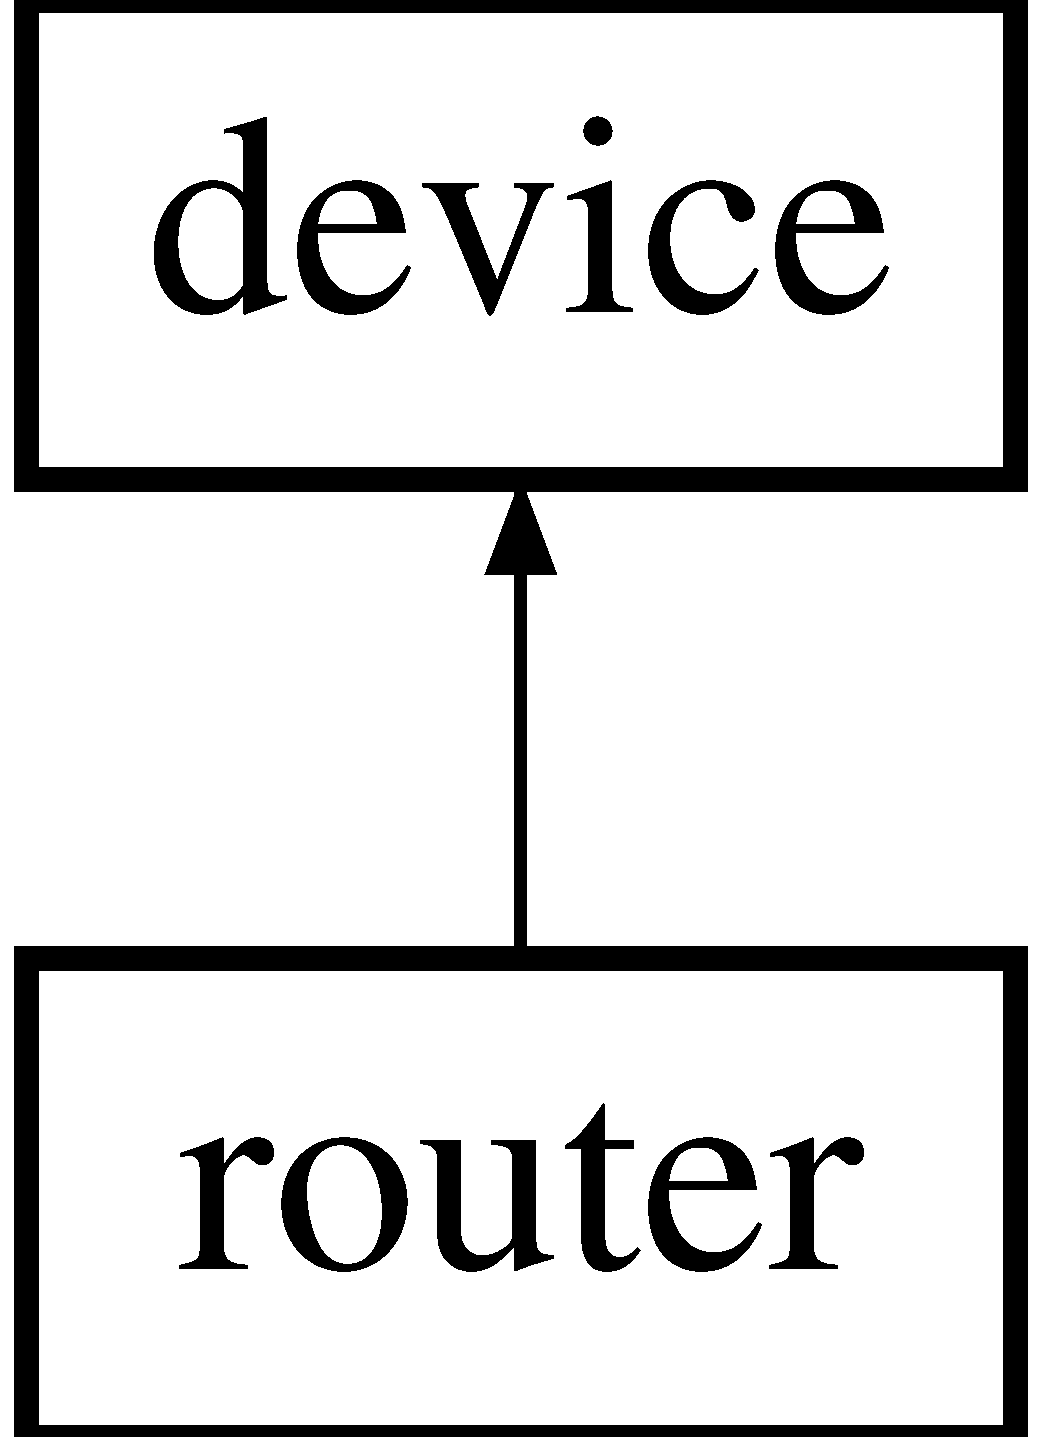
\includegraphics[height=2.000000cm]{classrouter}
\end{center}
\end{figure}
\subsection*{Public Member Functions}
\begin{DoxyCompactItemize}
\item 
\hyperlink{classrouter_af5559739f6e4f9b1c7f7bf80e32f6cd9}{router} ()
\begin{DoxyCompactList}\small\item\em Construct a router. \item\end{DoxyCompactList}\item 
\hyperlink{classrouter_a43d7888550284a3bffff71abf6c087eb}{router} (int, string, double, double, int, int)
\item 
\hyperlink{classrouter_a64870f29b48d6ee6276ec27b1b18e189}{$\sim$router} ()
\begin{DoxyCompactList}\small\item\em Destructor. \item\end{DoxyCompactList}\item 
list$<$ \hyperlink{classrLink}{rLink} $>$ \hyperlink{classrouter_a36115bd5923217c64922b2231f05c304}{getRListLink} ()
\begin{DoxyCompactList}\small\item\em Gets a router's link list. \item\end{DoxyCompactList}\item 
double \hyperlink{classrouter_a0c1d4a7689e992d90b0fcbf4a958c8b4}{getActualCapacity} ()
\begin{DoxyCompactList}\small\item\em Gets actual capacity of a router. \item\end{DoxyCompactList}\item 
double \hyperlink{classrouter_a7d5187977fd2dbf2fa562d3953647699}{getResidual} ()
\begin{DoxyCompactList}\small\item\em Gets residual capacity of a router. \item\end{DoxyCompactList}\item 
double \hyperlink{classrouter_a425b6d8372b0951a77097d0e6b49914a}{getTotalPower} ()
\begin{DoxyCompactList}\small\item\em Get total power of a router = router power + sum of power of the links there of. \item\end{DoxyCompactList}\item 
bool \hyperlink{classrouter_aaa3d78b2556a095f725d5a2202265d55}{getFlag} ()
\begin{DoxyCompactList}\small\item\em Gets if a flag is set or not. \item\end{DoxyCompactList}\item 
void \hyperlink{classrouter_a20f58c16edd3ca8d8afb73cf9f27f549}{setLList} (\hyperlink{classrLink}{rLink})
\begin{DoxyCompactList}\small\item\em Sets a router's link list. \item\end{DoxyCompactList}\item 
void \hyperlink{classrouter_a28908a05b7e50a0ab45481c94c8042a8}{setRLinkList} (list$<$ \hyperlink{classrLink}{rLink} $>$)
\begin{DoxyCompactList}\small\item\em Overwrite a router's link list if required after some modification. \item\end{DoxyCompactList}\item 
void \hyperlink{classrouter_a90c5339e7bed5597f06be903305ef588}{setActualCapacity} (double)
\begin{DoxyCompactList}\small\item\em Sets a router's capacity. \item\end{DoxyCompactList}\item 
void \hyperlink{classrouter_a9b06f4e341fea7bf5a853b0a2caf1d2a}{setTotalPower} (double)
\begin{DoxyCompactList}\small\item\em Sets a router's total power consumption = router power + sum of power consumption of links thereof. \item\end{DoxyCompactList}\item 
void \hyperlink{classrouter_ac839466bae2c42cee73a33b4d185f48a}{setResidual} (double)
\begin{DoxyCompactList}\small\item\em Sets residual capacity. \item\end{DoxyCompactList}\item 
void \hyperlink{classrouter_ab4e2af9a6d0412fa8d3e6cea8b411f7c}{setFlag} (bool)
\begin{DoxyCompactList}\small\item\em Sets/Resets router flag. \item\end{DoxyCompactList}\end{DoxyCompactItemize}


\subsection{Detailed Description}
Multistage architecture router class reference. It inherits device class and creates a new router with list of links in the same router.

{\bfseries Usage Example:} 
\begin{DoxyCode}
 router *r = new router(1, "router_1", 0, 0, 0, 0)
\end{DoxyCode}
 \begin{DoxySeeAlso}{See also}
\hyperlink{classdevice_a57b9c4ac7a8bd970b81b1154ae79a5de}{device(int ,string ,double ,double ,int ,int )} 
\end{DoxySeeAlso}


\subsection{Constructor \& Destructor Documentation}
\hypertarget{classrouter_af5559739f6e4f9b1c7f7bf80e32f6cd9}{
\index{router@{router}!router@{router}}
\index{router@{router}!router@{router}}
\subsubsection[{router}]{\setlength{\rightskip}{0pt plus 5cm}router::router (
\begin{DoxyParamCaption}
{}
\end{DoxyParamCaption}
)\hspace{0.3cm}{\ttfamily  \mbox{[}inline\mbox{]}}}}
\label{classrouter_af5559739f6e4f9b1c7f7bf80e32f6cd9}


Construct a router. 


\begin{DoxyParams}{Parameters}
\item[{\em ID}]router identification number \item[{\em name}]router name \item[{\em capacity}]router capacity \item[{\em power}]router power consumption \item[{\em nr\_\-links}]number of links contained inside a router \item[{\em state}]router state: ON/OFF \end{DoxyParams}
\begin{DoxySeeAlso}{See also}
\hyperlink{classdevice_a57b9c4ac7a8bd970b81b1154ae79a5de}{device(int ,string ,double ,double ,int ,int )} 
\end{DoxySeeAlso}
\hypertarget{classrouter_a43d7888550284a3bffff71abf6c087eb}{
\index{router@{router}!router@{router}}
\index{router@{router}!router@{router}}
\subsubsection[{router}]{\setlength{\rightskip}{0pt plus 5cm}router::router (
\begin{DoxyParamCaption}
\item[{int}]{ ID, }
\item[{string}]{ name, }
\item[{double}]{ capacity, }
\item[{double}]{ power, }
\item[{int}]{ state, }
\item[{int}]{ nr\_\-links}
\end{DoxyParamCaption}
)}}
\label{classrouter_a43d7888550284a3bffff71abf6c087eb}
\hypertarget{classrouter_a64870f29b48d6ee6276ec27b1b18e189}{
\index{router@{router}!$\sim$router@{$\sim$router}}
\index{$\sim$router@{$\sim$router}!router@{router}}
\subsubsection[{$\sim$router}]{\setlength{\rightskip}{0pt plus 5cm}router::$\sim$router (
\begin{DoxyParamCaption}
{}
\end{DoxyParamCaption}
)\hspace{0.3cm}{\ttfamily  \mbox{[}inline\mbox{]}}}}
\label{classrouter_a64870f29b48d6ee6276ec27b1b18e189}


Destructor. 



\subsection{Member Function Documentation}
\hypertarget{classrouter_a0c1d4a7689e992d90b0fcbf4a958c8b4}{
\index{router@{router}!getActualCapacity@{getActualCapacity}}
\index{getActualCapacity@{getActualCapacity}!router@{router}}
\subsubsection[{getActualCapacity}]{\setlength{\rightskip}{0pt plus 5cm}double router::getActualCapacity (
\begin{DoxyParamCaption}
{}
\end{DoxyParamCaption}
)}}
\label{classrouter_a0c1d4a7689e992d90b0fcbf4a958c8b4}


Gets actual capacity of a router. 

\begin{DoxyReturn}{Returns}
actual capacity of a router 
\end{DoxyReturn}
\hypertarget{classrouter_aaa3d78b2556a095f725d5a2202265d55}{
\index{router@{router}!getFlag@{getFlag}}
\index{getFlag@{getFlag}!router@{router}}
\subsubsection[{getFlag}]{\setlength{\rightskip}{0pt plus 5cm}bool router::getFlag (
\begin{DoxyParamCaption}
{}
\end{DoxyParamCaption}
)}}
\label{classrouter_aaa3d78b2556a095f725d5a2202265d55}


Gets if a flag is set or not. 

\begin{DoxyReturn}{Returns}
usage flag indicator 
\end{DoxyReturn}
\hypertarget{classrouter_a7d5187977fd2dbf2fa562d3953647699}{
\index{router@{router}!getResidual@{getResidual}}
\index{getResidual@{getResidual}!router@{router}}
\subsubsection[{getResidual}]{\setlength{\rightskip}{0pt plus 5cm}double router::getResidual (
\begin{DoxyParamCaption}
{}
\end{DoxyParamCaption}
)}}
\label{classrouter_a7d5187977fd2dbf2fa562d3953647699}


Gets residual capacity of a router. 

\begin{DoxyReturn}{Returns}
residual capacity of a router 
\end{DoxyReturn}
\hypertarget{classrouter_a36115bd5923217c64922b2231f05c304}{
\index{router@{router}!getRListLink@{getRListLink}}
\index{getRListLink@{getRListLink}!router@{router}}
\subsubsection[{getRListLink}]{\setlength{\rightskip}{0pt plus 5cm}list$<$ {\bf rLink} $>$ router::getRListLink (
\begin{DoxyParamCaption}
{}
\end{DoxyParamCaption}
)}}
\label{classrouter_a36115bd5923217c64922b2231f05c304}


Gets a router's link list. 

\begin{DoxyReturn}{Returns}
list of links on a router 
\end{DoxyReturn}
\hypertarget{classrouter_a425b6d8372b0951a77097d0e6b49914a}{
\index{router@{router}!getTotalPower@{getTotalPower}}
\index{getTotalPower@{getTotalPower}!router@{router}}
\subsubsection[{getTotalPower}]{\setlength{\rightskip}{0pt plus 5cm}double router::getTotalPower (
\begin{DoxyParamCaption}
{}
\end{DoxyParamCaption}
)}}
\label{classrouter_a425b6d8372b0951a77097d0e6b49914a}


Get total power of a router = router power + sum of power of the links there of. 

\begin{DoxyReturn}{Returns}
total power of a router 
\end{DoxyReturn}
\hypertarget{classrouter_a90c5339e7bed5597f06be903305ef588}{
\index{router@{router}!setActualCapacity@{setActualCapacity}}
\index{setActualCapacity@{setActualCapacity}!router@{router}}
\subsubsection[{setActualCapacity}]{\setlength{\rightskip}{0pt plus 5cm}void router::setActualCapacity (
\begin{DoxyParamCaption}
\item[{double}]{ actualCapacity}
\end{DoxyParamCaption}
)}}
\label{classrouter_a90c5339e7bed5597f06be903305ef588}


Sets a router's capacity. 


\begin{DoxyParams}{Parameters}
\item[{\em actualCapacity}]router capacity \end{DoxyParams}
\hypertarget{classrouter_ab4e2af9a6d0412fa8d3e6cea8b411f7c}{
\index{router@{router}!setFlag@{setFlag}}
\index{setFlag@{setFlag}!router@{router}}
\subsubsection[{setFlag}]{\setlength{\rightskip}{0pt plus 5cm}void router::setFlag (
\begin{DoxyParamCaption}
\item[{bool}]{ flag}
\end{DoxyParamCaption}
)}}
\label{classrouter_ab4e2af9a6d0412fa8d3e6cea8b411f7c}


Sets/Resets router flag. 


\begin{DoxyParams}{Parameters}
\item[{\em flag}]a boolean value: 1 if the router is used in routing operation, 0 otherwise \end{DoxyParams}
\hypertarget{classrouter_a20f58c16edd3ca8d8afb73cf9f27f549}{
\index{router@{router}!setLList@{setLList}}
\index{setLList@{setLList}!router@{router}}
\subsubsection[{setLList}]{\setlength{\rightskip}{0pt plus 5cm}void router::setLList (
\begin{DoxyParamCaption}
\item[{{\bf rLink}}]{ l}
\end{DoxyParamCaption}
)}}
\label{classrouter_a20f58c16edd3ca8d8afb73cf9f27f549}


Sets a router's link list. 


\begin{DoxyParams}{Parameters}
\item[{\em l}]link with all its attributes \end{DoxyParams}
\hypertarget{classrouter_ac839466bae2c42cee73a33b4d185f48a}{
\index{router@{router}!setResidual@{setResidual}}
\index{setResidual@{setResidual}!router@{router}}
\subsubsection[{setResidual}]{\setlength{\rightskip}{0pt plus 5cm}void router::setResidual (
\begin{DoxyParamCaption}
\item[{double}]{ residual}
\end{DoxyParamCaption}
)}}
\label{classrouter_ac839466bae2c42cee73a33b4d185f48a}


Sets residual capacity. 


\begin{DoxyParams}{Parameters}
\item[{\em residual}]\end{DoxyParams}
\hypertarget{classrouter_a28908a05b7e50a0ab45481c94c8042a8}{
\index{router@{router}!setRLinkList@{setRLinkList}}
\index{setRLinkList@{setRLinkList}!router@{router}}
\subsubsection[{setRLinkList}]{\setlength{\rightskip}{0pt plus 5cm}void router::setRLinkList (
\begin{DoxyParamCaption}
\item[{list$<$ {\bf rLink} $>$}]{ lList}
\end{DoxyParamCaption}
)}}
\label{classrouter_a28908a05b7e50a0ab45481c94c8042a8}


Overwrite a router's link list if required after some modification. 


\begin{DoxyParams}{Parameters}
\item[{\em lList}]link list \end{DoxyParams}
\hypertarget{classrouter_a9b06f4e341fea7bf5a853b0a2caf1d2a}{
\index{router@{router}!setTotalPower@{setTotalPower}}
\index{setTotalPower@{setTotalPower}!router@{router}}
\subsubsection[{setTotalPower}]{\setlength{\rightskip}{0pt plus 5cm}void router::setTotalPower (
\begin{DoxyParamCaption}
\item[{double}]{ totalP}
\end{DoxyParamCaption}
)}}
\label{classrouter_a9b06f4e341fea7bf5a853b0a2caf1d2a}


Sets a router's total power consumption = router power + sum of power consumption of links thereof. 


\begin{DoxyParams}{Parameters}
\item[{\em totalP}]total power consumption of a router \end{DoxyParams}


The documentation for this class was generated from the following files:\begin{DoxyCompactItemize}
\item 
/home/fikru/Desktop/fikru/research/code/online\_\-energy\_\-saving\_\-splittable/include/\hyperlink{router_8h}{router.h}\item 
/home/fikru/Desktop/fikru/research/code/online\_\-energy\_\-saving\_\-splittable/\hyperlink{router_8cpp}{router.cpp}\end{DoxyCompactItemize}

\hypertarget{classstatistics}{
\section{statistics Class Reference}
\label{classstatistics}\index{statistics@{statistics}}
}


Statistics class to collect device states.  




{\ttfamily \#include $<$statistics.h$>$}

\subsection*{Public Member Functions}
\begin{DoxyCompactItemize}
\item 
\hyperlink{classstatistics_a31d6750c3251c979f5c2d013984e1162}{statistics} ()
\begin{DoxyCompactList}\small\item\em constructor \item\end{DoxyCompactList}\item 
\hyperlink{classstatistics_a8cf720227802726be118712dc6616f94}{$\sim$statistics} ()
\begin{DoxyCompactList}\small\item\em destructor \item\end{DoxyCompactList}\item 
std::vector$<$ double $>$ \hyperlink{classstatistics_ab2c51b1a4cc826a09473860faf565360}{getForwardedList} ()
\begin{DoxyCompactList}\small\item\em get forwarded traffic list \item\end{DoxyCompactList}\item 
std::vector$<$ double $>$ \hyperlink{classstatistics_a99795974e97556668c02c5005b2df895}{getLostList} ()
\begin{DoxyCompactList}\small\item\em get lost traffic list \item\end{DoxyCompactList}\item 
std::vector$<$ long $>$ \hyperlink{classstatistics_aabf7c631faf37c1c75435b94b364b7b0}{getTimeAdvList} ()
\begin{DoxyCompactList}\small\item\em get advanced time \item\end{DoxyCompactList}\item 
std::vector$<$ double $>$ \hyperlink{classstatistics_a47b6c911143330c41faa573bc534aee1}{getObjectiveList} ()
\begin{DoxyCompactList}\small\item\em get objective \item\end{DoxyCompactList}\item 
std::vector$<$ double $>$ \hyperlink{classstatistics_a170d529ea5d3c459755309e2de1d166e}{getLoadList} ()
\begin{DoxyCompactList}\small\item\em get load \item\end{DoxyCompactList}\item 
double \hyperlink{classstatistics_a8a09566df54f2ac183e0a40f452546a6}{getObjective} ()
\begin{DoxyCompactList}\small\item\em get objective previous \item\end{DoxyCompactList}\item 
void \hyperlink{classstatistics_a94f979fcc6d511583638d6fc12116992}{setForwardedList} (double)
\begin{DoxyCompactList}\small\item\em set forwarded traffic list \item\end{DoxyCompactList}\item 
void \hyperlink{classstatistics_a84bead3d62e23af1777b5e54c6de48de}{setLostList} (double)
\begin{DoxyCompactList}\small\item\em set lost traffic list \item\end{DoxyCompactList}\item 
void \hyperlink{classstatistics_ad738c092d2d09223d4c9853c2859d7cd}{setTimeAdvList} (long)
\begin{DoxyCompactList}\small\item\em set advanced time \item\end{DoxyCompactList}\item 
void \hyperlink{classstatistics_ab2fd434123379e7814c21bc38ff2bb20}{setObjective} (double)
\begin{DoxyCompactList}\small\item\em set current objective \item\end{DoxyCompactList}\item 
void \hyperlink{classstatistics_a625258dee0b4eaf0fa5ade3643a4535e}{setObjectiveList} (double)
\begin{DoxyCompactList}\small\item\em put objective in the list \item\end{DoxyCompactList}\item 
void \hyperlink{classstatistics_af1594f7585e2c0776ef2f8fb7ddd3fca}{setLoadList} (double)
\begin{DoxyCompactList}\small\item\em set load \item\end{DoxyCompactList}\end{DoxyCompactItemize}


\subsection{Detailed Description}
Statistics class to collect device states. General traffic statistics -\/ such as lost traffic, total forwarded traffic, total power consumption (objective) 

\subsection{Constructor \& Destructor Documentation}
\hypertarget{classstatistics_a31d6750c3251c979f5c2d013984e1162}{
\index{statistics@{statistics}!statistics@{statistics}}
\index{statistics@{statistics}!statistics@{statistics}}
\subsubsection[{statistics}]{\setlength{\rightskip}{0pt plus 5cm}statistics::statistics (
\begin{DoxyParamCaption}
{}
\end{DoxyParamCaption}
)}}
\label{classstatistics_a31d6750c3251c979f5c2d013984e1162}


constructor 

\hypertarget{classstatistics_a8cf720227802726be118712dc6616f94}{
\index{statistics@{statistics}!$\sim$statistics@{$\sim$statistics}}
\index{$\sim$statistics@{$\sim$statistics}!statistics@{statistics}}
\subsubsection[{$\sim$statistics}]{\setlength{\rightskip}{0pt plus 5cm}statistics::$\sim$statistics (
\begin{DoxyParamCaption}
{}
\end{DoxyParamCaption}
)\hspace{0.3cm}{\ttfamily  \mbox{[}inline\mbox{]}}}}
\label{classstatistics_a8cf720227802726be118712dc6616f94}


destructor 



\subsection{Member Function Documentation}
\hypertarget{classstatistics_ab2c51b1a4cc826a09473860faf565360}{
\index{statistics@{statistics}!getForwardedList@{getForwardedList}}
\index{getForwardedList@{getForwardedList}!statistics@{statistics}}
\subsubsection[{getForwardedList}]{\setlength{\rightskip}{0pt plus 5cm}std::vector$<$ double $>$ statistics::getForwardedList (
\begin{DoxyParamCaption}
{}
\end{DoxyParamCaption}
)}}
\label{classstatistics_ab2c51b1a4cc826a09473860faf565360}


get forwarded traffic list 

\begin{DoxyReturn}{Returns}
forwarded traffic list 
\end{DoxyReturn}
\hypertarget{classstatistics_a170d529ea5d3c459755309e2de1d166e}{
\index{statistics@{statistics}!getLoadList@{getLoadList}}
\index{getLoadList@{getLoadList}!statistics@{statistics}}
\subsubsection[{getLoadList}]{\setlength{\rightskip}{0pt plus 5cm}std::vector$<$ double $>$ statistics::getLoadList (
\begin{DoxyParamCaption}
{}
\end{DoxyParamCaption}
)}}
\label{classstatistics_a170d529ea5d3c459755309e2de1d166e}


get load 

\begin{DoxyReturn}{Returns}
list of loads 
\end{DoxyReturn}
\hypertarget{classstatistics_a99795974e97556668c02c5005b2df895}{
\index{statistics@{statistics}!getLostList@{getLostList}}
\index{getLostList@{getLostList}!statistics@{statistics}}
\subsubsection[{getLostList}]{\setlength{\rightskip}{0pt plus 5cm}std::vector$<$ double $>$ statistics::getLostList (
\begin{DoxyParamCaption}
{}
\end{DoxyParamCaption}
)}}
\label{classstatistics_a99795974e97556668c02c5005b2df895}


get lost traffic list 

\begin{DoxyReturn}{Returns}
lost traffic list 
\end{DoxyReturn}
\hypertarget{classstatistics_a8a09566df54f2ac183e0a40f452546a6}{
\index{statistics@{statistics}!getObjective@{getObjective}}
\index{getObjective@{getObjective}!statistics@{statistics}}
\subsubsection[{getObjective}]{\setlength{\rightskip}{0pt plus 5cm}double statistics::getObjective (
\begin{DoxyParamCaption}
{}
\end{DoxyParamCaption}
)}}
\label{classstatistics_a8a09566df54f2ac183e0a40f452546a6}


get objective previous 

\begin{DoxyReturn}{Returns}
total power consumption of the previous configuration of the architecture 
\end{DoxyReturn}
\hypertarget{classstatistics_a47b6c911143330c41faa573bc534aee1}{
\index{statistics@{statistics}!getObjectiveList@{getObjectiveList}}
\index{getObjectiveList@{getObjectiveList}!statistics@{statistics}}
\subsubsection[{getObjectiveList}]{\setlength{\rightskip}{0pt plus 5cm}std::vector$<$ double $>$ statistics::getObjectiveList (
\begin{DoxyParamCaption}
{}
\end{DoxyParamCaption}
)}}
\label{classstatistics_a47b6c911143330c41faa573bc534aee1}


get objective 

\begin{DoxyReturn}{Returns}
list of total power consumption of the architecture 
\end{DoxyReturn}
\hypertarget{classstatistics_aabf7c631faf37c1c75435b94b364b7b0}{
\index{statistics@{statistics}!getTimeAdvList@{getTimeAdvList}}
\index{getTimeAdvList@{getTimeAdvList}!statistics@{statistics}}
\subsubsection[{getTimeAdvList}]{\setlength{\rightskip}{0pt plus 5cm}std::vector$<$ long $>$ statistics::getTimeAdvList (
\begin{DoxyParamCaption}
{}
\end{DoxyParamCaption}
)}}
\label{classstatistics_aabf7c631faf37c1c75435b94b364b7b0}


get advanced time 

\begin{DoxyReturn}{Returns}
time required for packing 
\end{DoxyReturn}
\hypertarget{classstatistics_a94f979fcc6d511583638d6fc12116992}{
\index{statistics@{statistics}!setForwardedList@{setForwardedList}}
\index{setForwardedList@{setForwardedList}!statistics@{statistics}}
\subsubsection[{setForwardedList}]{\setlength{\rightskip}{0pt plus 5cm}void statistics::setForwardedList (
\begin{DoxyParamCaption}
\item[{double}]{ forwarded}
\end{DoxyParamCaption}
)}}
\label{classstatistics_a94f979fcc6d511583638d6fc12116992}


set forwarded traffic list 


\begin{DoxyParams}{Parameters}
\item[{\em forwarded}]routed traffic \end{DoxyParams}
\hypertarget{classstatistics_af1594f7585e2c0776ef2f8fb7ddd3fca}{
\index{statistics@{statistics}!setLoadList@{setLoadList}}
\index{setLoadList@{setLoadList}!statistics@{statistics}}
\subsubsection[{setLoadList}]{\setlength{\rightskip}{0pt plus 5cm}void statistics::setLoadList (
\begin{DoxyParamCaption}
\item[{double}]{ load}
\end{DoxyParamCaption}
)}}
\label{classstatistics_af1594f7585e2c0776ef2f8fb7ddd3fca}


set load 


\begin{DoxyParams}{Parameters}
\item[{\em load}]current traffic amount to be forwarded \end{DoxyParams}
\hypertarget{classstatistics_a84bead3d62e23af1777b5e54c6de48de}{
\index{statistics@{statistics}!setLostList@{setLostList}}
\index{setLostList@{setLostList}!statistics@{statistics}}
\subsubsection[{setLostList}]{\setlength{\rightskip}{0pt plus 5cm}void statistics::setLostList (
\begin{DoxyParamCaption}
\item[{double}]{ lost}
\end{DoxyParamCaption}
)}}
\label{classstatistics_a84bead3d62e23af1777b5e54c6de48de}


set lost traffic list 


\begin{DoxyParams}{Parameters}
\item[{\em lost}]traffic that is not routed because of lack of capacity \end{DoxyParams}
\hypertarget{classstatistics_ab2fd434123379e7814c21bc38ff2bb20}{
\index{statistics@{statistics}!setObjective@{setObjective}}
\index{setObjective@{setObjective}!statistics@{statistics}}
\subsubsection[{setObjective}]{\setlength{\rightskip}{0pt plus 5cm}void statistics::setObjective (
\begin{DoxyParamCaption}
\item[{double}]{ objective}
\end{DoxyParamCaption}
)}}
\label{classstatistics_ab2fd434123379e7814c21bc38ff2bb20}


set current objective 


\begin{DoxyParams}{Parameters}
\item[{\em objective}]power consumption of current configuration \end{DoxyParams}
\hypertarget{classstatistics_a625258dee0b4eaf0fa5ade3643a4535e}{
\index{statistics@{statistics}!setObjectiveList@{setObjectiveList}}
\index{setObjectiveList@{setObjectiveList}!statistics@{statistics}}
\subsubsection[{setObjectiveList}]{\setlength{\rightskip}{0pt plus 5cm}void statistics::setObjectiveList (
\begin{DoxyParamCaption}
\item[{double}]{ objective}
\end{DoxyParamCaption}
)}}
\label{classstatistics_a625258dee0b4eaf0fa5ade3643a4535e}


put objective in the list 


\begin{DoxyParams}{Parameters}
\item[{\em objective}]power consumption of current configuration \end{DoxyParams}
\hypertarget{classstatistics_ad738c092d2d09223d4c9853c2859d7cd}{
\index{statistics@{statistics}!setTimeAdvList@{setTimeAdvList}}
\index{setTimeAdvList@{setTimeAdvList}!statistics@{statistics}}
\subsubsection[{setTimeAdvList}]{\setlength{\rightskip}{0pt plus 5cm}void statistics::setTimeAdvList (
\begin{DoxyParamCaption}
\item[{long}]{ time\_\-adv}
\end{DoxyParamCaption}
)}}
\label{classstatistics_ad738c092d2d09223d4c9853c2859d7cd}


set advanced time 


\begin{DoxyParams}{Parameters}
\item[{\em time\_\-adv}]time since the beginning of running the heuristic \end{DoxyParams}


The documentation for this class was generated from the following files:\begin{DoxyCompactItemize}
\item 
/home/fikru/Desktop/fikru/research/code/online\_\-energy\_\-saving\_\-splittable/include/\hyperlink{statistics_8h}{statistics.h}\item 
/home/fikru/Desktop/fikru/research/code/online\_\-energy\_\-saving\_\-splittable/\hyperlink{statistics_8cpp}{statistics.cpp}\end{DoxyCompactItemize}

\hypertarget{classtimer}{
\section{timer Class Reference}
\label{classtimer}\index{timer@{timer}}
}


Basic class to calculate time difference.  




{\ttfamily \#include $<$timer.h$>$}

\subsection*{Public Member Functions}
\begin{DoxyCompactItemize}
\item 
\hyperlink{classtimer_ae536faf93e02933cd025a6fbcbb48d0a}{timer} ()
\begin{DoxyCompactList}\small\item\em constructor \item\end{DoxyCompactList}\item 
\hyperlink{classtimer_aee05958ea6b0fbf36ea1fd22747cd546}{$\sim$timer} ()
\begin{DoxyCompactList}\small\item\em destructor \item\end{DoxyCompactList}\item 
void \hyperlink{classtimer_ac5b8fb9779cf72c599d3360a75bc5b89}{setStart} ()
\begin{DoxyCompactList}\small\item\em saves the beginning of the simulation run \item\end{DoxyCompactList}\item 
void \hyperlink{classtimer_ae666e8e84f8ccccd1280518bc7c3f9c0}{setEnd} ()
\begin{DoxyCompactList}\small\item\em saves the end of the simulation run \item\end{DoxyCompactList}\item 
timeval \hyperlink{classtimer_aad52287ca6d6a3a285e171a592a85847}{getStart} ()
\begin{DoxyCompactList}\small\item\em get simulation start time \item\end{DoxyCompactList}\item 
timeval \hyperlink{classtimer_aa415a63f52ee3efb36bbeb9d18a813b8}{getEnd} ()
\begin{DoxyCompactList}\small\item\em get simulation end time \item\end{DoxyCompactList}\end{DoxyCompactItemize}


\subsection{Detailed Description}
Basic class to calculate time difference. 

\subsection{Constructor \& Destructor Documentation}
\hypertarget{classtimer_ae536faf93e02933cd025a6fbcbb48d0a}{
\index{timer@{timer}!timer@{timer}}
\index{timer@{timer}!timer@{timer}}
\subsubsection[{timer}]{\setlength{\rightskip}{0pt plus 5cm}timer::timer (
\begin{DoxyParamCaption}
{}
\end{DoxyParamCaption}
)}}
\label{classtimer_ae536faf93e02933cd025a6fbcbb48d0a}


constructor 

\hypertarget{classtimer_aee05958ea6b0fbf36ea1fd22747cd546}{
\index{timer@{timer}!$\sim$timer@{$\sim$timer}}
\index{$\sim$timer@{$\sim$timer}!timer@{timer}}
\subsubsection[{$\sim$timer}]{\setlength{\rightskip}{0pt plus 5cm}timer::$\sim$timer (
\begin{DoxyParamCaption}
{}
\end{DoxyParamCaption}
)}}
\label{classtimer_aee05958ea6b0fbf36ea1fd22747cd546}


destructor 



\subsection{Member Function Documentation}
\hypertarget{classtimer_aa415a63f52ee3efb36bbeb9d18a813b8}{
\index{timer@{timer}!getEnd@{getEnd}}
\index{getEnd@{getEnd}!timer@{timer}}
\subsubsection[{getEnd}]{\setlength{\rightskip}{0pt plus 5cm}timeval timer::getEnd (
\begin{DoxyParamCaption}
{}
\end{DoxyParamCaption}
)}}
\label{classtimer_aa415a63f52ee3efb36bbeb9d18a813b8}


get simulation end time 

\begin{DoxyReturn}{Returns}
simulation end time -\/ since epoch time 
\end{DoxyReturn}
\hypertarget{classtimer_aad52287ca6d6a3a285e171a592a85847}{
\index{timer@{timer}!getStart@{getStart}}
\index{getStart@{getStart}!timer@{timer}}
\subsubsection[{getStart}]{\setlength{\rightskip}{0pt plus 5cm}timeval timer::getStart (
\begin{DoxyParamCaption}
{}
\end{DoxyParamCaption}
)}}
\label{classtimer_aad52287ca6d6a3a285e171a592a85847}


get simulation start time 

\begin{DoxyReturn}{Returns}
simulation start time -\/ since epoch time 
\end{DoxyReturn}
\hypertarget{classtimer_ae666e8e84f8ccccd1280518bc7c3f9c0}{
\index{timer@{timer}!setEnd@{setEnd}}
\index{setEnd@{setEnd}!timer@{timer}}
\subsubsection[{setEnd}]{\setlength{\rightskip}{0pt plus 5cm}void timer::setEnd (
\begin{DoxyParamCaption}
{}
\end{DoxyParamCaption}
)}}
\label{classtimer_ae666e8e84f8ccccd1280518bc7c3f9c0}


saves the end of the simulation run 

\hypertarget{classtimer_ac5b8fb9779cf72c599d3360a75bc5b89}{
\index{timer@{timer}!setStart@{setStart}}
\index{setStart@{setStart}!timer@{timer}}
\subsubsection[{setStart}]{\setlength{\rightskip}{0pt plus 5cm}void timer::setStart (
\begin{DoxyParamCaption}
{}
\end{DoxyParamCaption}
)}}
\label{classtimer_ac5b8fb9779cf72c599d3360a75bc5b89}


saves the beginning of the simulation run 



The documentation for this class was generated from the following files:\begin{DoxyCompactItemize}
\item 
/home/fikru/Desktop/fikru/research/code/online\_\-energy\_\-saving\_\-splittable/include/\hyperlink{timer_8h}{timer.h}\item 
/home/fikru/Desktop/fikru/research/code/online\_\-energy\_\-saving\_\-splittable/\hyperlink{timer_8cpp}{timer.cpp}\end{DoxyCompactItemize}

\hypertarget{classtrafficgen}{
\section{trafficgen Class Reference}
\label{classtrafficgen}\index{trafficgen@{trafficgen}}
}


Traffic generator.  




{\ttfamily \#include $<$trafficgen.h$>$}

\subsection*{Public Member Functions}
\begin{DoxyCompactItemize}
\item 
\hyperlink{classtrafficgen_a5dff07c6da8f8b999ddaea3f66f35f97}{trafficgen} ()
\begin{DoxyCompactList}\small\item\em constructor \item\end{DoxyCompactList}\item 
\hyperlink{classtrafficgen_ac354957233749112711e372977013674}{$\sim$trafficgen} ()
\begin{DoxyCompactList}\small\item\em destructor \item\end{DoxyCompactList}\item 
double \hyperlink{classtrafficgen_ab91f6ea4b48657844b9c925d3d1c8466}{setLoad} (double, double, long $\ast$)
\begin{DoxyCompactList}\small\item\em sets and return a new load \item\end{DoxyCompactList}\end{DoxyCompactItemize}


\subsection{Detailed Description}
Traffic generator. Generate a uniformly distributed traffic load in a given range. The maximum is set to the architecture capacity 

\subsection{Constructor \& Destructor Documentation}
\hypertarget{classtrafficgen_a5dff07c6da8f8b999ddaea3f66f35f97}{
\index{trafficgen@{trafficgen}!trafficgen@{trafficgen}}
\index{trafficgen@{trafficgen}!trafficgen@{trafficgen}}
\subsubsection[{trafficgen}]{\setlength{\rightskip}{0pt plus 5cm}trafficgen::trafficgen (
\begin{DoxyParamCaption}
{}
\end{DoxyParamCaption}
)}}
\label{classtrafficgen_a5dff07c6da8f8b999ddaea3f66f35f97}


constructor 

\hypertarget{classtrafficgen_ac354957233749112711e372977013674}{
\index{trafficgen@{trafficgen}!$\sim$trafficgen@{$\sim$trafficgen}}
\index{$\sim$trafficgen@{$\sim$trafficgen}!trafficgen@{trafficgen}}
\subsubsection[{$\sim$trafficgen}]{\setlength{\rightskip}{0pt plus 5cm}trafficgen::$\sim$trafficgen (
\begin{DoxyParamCaption}
{}
\end{DoxyParamCaption}
)}}
\label{classtrafficgen_ac354957233749112711e372977013674}


destructor 



\subsection{Member Function Documentation}
\hypertarget{classtrafficgen_ab91f6ea4b48657844b9c925d3d1c8466}{
\index{trafficgen@{trafficgen}!setLoad@{setLoad}}
\index{setLoad@{setLoad}!trafficgen@{trafficgen}}
\subsubsection[{setLoad}]{\setlength{\rightskip}{0pt plus 5cm}double trafficgen::setLoad (
\begin{DoxyParamCaption}
\item[{double}]{ min, }
\item[{double}]{ max, }
\item[{long $\ast$}]{ seed}
\end{DoxyParamCaption}
)}}
\label{classtrafficgen_ab91f6ea4b48657844b9c925d3d1c8466}


sets and return a new load 


\begin{DoxyParams}{Parameters}
\item[{\em min}]the minimum traffic = 0 \item[{\em max}]the maximum traffic = the maximum architecture capacity \item[{\em seed}]to seed the random generator \end{DoxyParams}
\begin{DoxyReturn}{Returns}
lLoad current trafic load 
\end{DoxyReturn}


The documentation for this class was generated from the following files:\begin{DoxyCompactItemize}
\item 
/home/fikru/Desktop/fikru/research/code/online\_\-energy\_\-saving\_\-splittable/include/\hyperlink{trafficgen_8h}{trafficgen.h}\item 
/home/fikru/Desktop/fikru/research/code/online\_\-energy\_\-saving\_\-splittable/\hyperlink{trafficgen_8cpp}{trafficgen.cpp}\end{DoxyCompactItemize}

\chapter{File Documentation}
\hypertarget{bin__packing_8cpp}{
\section{/home/fikru/Desktop/fikru/research/code/online\_\-energy\_\-saving\_\-splittable/bin\_\-packing.cpp File Reference}
\label{bin__packing_8cpp}\index{/home/fikru/Desktop/fikru/research/code/online\_\-energy\_\-saving\_\-splittable/bin\_\-packing.cpp@{/home/fikru/Desktop/fikru/research/code/online\_\-energy\_\-saving\_\-splittable/bin\_\-packing.cpp}}
}
{\ttfamily \#include $<$limits$>$}\par
{\ttfamily \#include \char`\"{}global.h\char`\"{}}\par
{\ttfamily \#include \char`\"{}rLink.h\char`\"{}}\par
{\ttfamily \#include $<$iostream$>$}\par
\subsection*{Functions}
\begin{DoxyCompactItemize}
\item 
void \hyperlink{bin__packing_8cpp_ad78939de31d26895a7f3816246ef9f04}{pack\_\-routers} (double \&, \hyperlink{classrouter}{router} \&)
\item 
void \hyperlink{bin__packing_8cpp_af26d02197ba7bd14a5584d766842dd21}{pack\_\-links} (double \&, \hyperlink{classrLink}{rLink} \&)
\item 
\hyperlink{classstatistics}{statistics} \hyperlink{bin__packing_8cpp_a63baeeb26318ce6be17ab91f4dcbd8fa}{bin\_\-packing} (double load\_\-leftover, list$<$ \hyperlink{classrouter}{router} $>$ \&\hyperlink{SCESApplication_8cpp_aae066c5ae750629985dad2d59db3de5a}{rList})
\item 
void \hyperlink{bin__packing_8cpp_ab6a031122ec81ed5fce4209bf1050aa9}{ff} (double load\_\-leftover, list$<$ \hyperlink{classrouter}{router} $>$ \&\hyperlink{SCESApplication_8cpp_aae066c5ae750629985dad2d59db3de5a}{rList})
\end{DoxyCompactItemize}
\subsection*{Variables}
\begin{DoxyCompactItemize}
\item 
int \hyperlink{bin__packing_8cpp_a86c9f04bfa1c110f70a46348b7f9e557}{objective}
\item 
bool \hyperlink{bin__packing_8cpp_a6793a4125be91b59e503672eaae9acd5}{packed\_\-flag}
\item 
bool \hyperlink{bin__packing_8cpp_a996c583417c1ec6c2bf4396af0eaa0c5}{lpacked\_\-flag}
\item 
int \hyperlink{bin__packing_8cpp_ad669c198cf8b952ad5877c1addfb7c78}{nr\_\-r}
\begin{DoxyCompactList}\small\item\em nr of routers used in current configuration \item\end{DoxyCompactList}\end{DoxyCompactItemize}


\subsection{Function Documentation}
\hypertarget{bin__packing_8cpp_a63baeeb26318ce6be17ab91f4dcbd8fa}{
\index{bin\_\-packing.cpp@{bin\_\-packing.cpp}!bin\_\-packing@{bin\_\-packing}}
\index{bin\_\-packing@{bin\_\-packing}!bin_packing.cpp@{bin\_\-packing.cpp}}
\subsubsection[{bin\_\-packing}]{\setlength{\rightskip}{0pt plus 5cm}{\bf statistics} bin\_\-packing (
\begin{DoxyParamCaption}
\item[{double}]{ load\_\-leftover, }
\item[{list$<$ {\bf router} $>$ \&}]{ rList}
\end{DoxyParamCaption}
)}}
\label{bin__packing_8cpp_a63baeeb26318ce6be17ab91f4dcbd8fa}
\hypertarget{bin__packing_8cpp_ab6a031122ec81ed5fce4209bf1050aa9}{
\index{bin\_\-packing.cpp@{bin\_\-packing.cpp}!ff@{ff}}
\index{ff@{ff}!bin_packing.cpp@{bin\_\-packing.cpp}}
\subsubsection[{ff}]{\setlength{\rightskip}{0pt plus 5cm}void ff (
\begin{DoxyParamCaption}
\item[{double}]{ load\_\-leftover, }
\item[{list$<$ {\bf router} $>$ \&}]{ rList}
\end{DoxyParamCaption}
)}}
\label{bin__packing_8cpp_ab6a031122ec81ed5fce4209bf1050aa9}
\hypertarget{bin__packing_8cpp_af26d02197ba7bd14a5584d766842dd21}{
\index{bin\_\-packing.cpp@{bin\_\-packing.cpp}!pack\_\-links@{pack\_\-links}}
\index{pack\_\-links@{pack\_\-links}!bin_packing.cpp@{bin\_\-packing.cpp}}
\subsubsection[{pack\_\-links}]{\setlength{\rightskip}{0pt plus 5cm}void pack\_\-links (
\begin{DoxyParamCaption}
\item[{double \&}]{ load, }
\item[{{\bf rLink} \&}]{ l\_\-itr}
\end{DoxyParamCaption}
)}}
\label{bin__packing_8cpp_af26d02197ba7bd14a5584d766842dd21}
\hypertarget{bin__packing_8cpp_ad78939de31d26895a7f3816246ef9f04}{
\index{bin\_\-packing.cpp@{bin\_\-packing.cpp}!pack\_\-routers@{pack\_\-routers}}
\index{pack\_\-routers@{pack\_\-routers}!bin_packing.cpp@{bin\_\-packing.cpp}}
\subsubsection[{pack\_\-routers}]{\setlength{\rightskip}{0pt plus 5cm}void pack\_\-routers (
\begin{DoxyParamCaption}
\item[{double \&}]{ load\_\-leftover, }
\item[{{\bf router} \&}]{ r\_\-itr}
\end{DoxyParamCaption}
)}}
\label{bin__packing_8cpp_ad78939de31d26895a7f3816246ef9f04}


\subsection{Variable Documentation}
\hypertarget{bin__packing_8cpp_a996c583417c1ec6c2bf4396af0eaa0c5}{
\index{bin\_\-packing.cpp@{bin\_\-packing.cpp}!lpacked\_\-flag@{lpacked\_\-flag}}
\index{lpacked\_\-flag@{lpacked\_\-flag}!bin_packing.cpp@{bin\_\-packing.cpp}}
\subsubsection[{lpacked\_\-flag}]{\setlength{\rightskip}{0pt plus 5cm}bool {\bf lpacked\_\-flag}}}
\label{bin__packing_8cpp_a996c583417c1ec6c2bf4396af0eaa0c5}
\hypertarget{bin__packing_8cpp_ad669c198cf8b952ad5877c1addfb7c78}{
\index{bin\_\-packing.cpp@{bin\_\-packing.cpp}!nr\_\-r@{nr\_\-r}}
\index{nr\_\-r@{nr\_\-r}!bin_packing.cpp@{bin\_\-packing.cpp}}
\subsubsection[{nr\_\-r}]{\setlength{\rightskip}{0pt plus 5cm}int {\bf nr\_\-r}}}
\label{bin__packing_8cpp_ad669c198cf8b952ad5877c1addfb7c78}


nr of routers used in current configuration 

\hypertarget{bin__packing_8cpp_a86c9f04bfa1c110f70a46348b7f9e557}{
\index{bin\_\-packing.cpp@{bin\_\-packing.cpp}!objective@{objective}}
\index{objective@{objective}!bin_packing.cpp@{bin\_\-packing.cpp}}
\subsubsection[{objective}]{\setlength{\rightskip}{0pt plus 5cm}int {\bf objective}}}
\label{bin__packing_8cpp_a86c9f04bfa1c110f70a46348b7f9e557}
\hypertarget{bin__packing_8cpp_a6793a4125be91b59e503672eaae9acd5}{
\index{bin\_\-packing.cpp@{bin\_\-packing.cpp}!packed\_\-flag@{packed\_\-flag}}
\index{packed\_\-flag@{packed\_\-flag}!bin_packing.cpp@{bin\_\-packing.cpp}}
\subsubsection[{packed\_\-flag}]{\setlength{\rightskip}{0pt plus 5cm}bool {\bf packed\_\-flag}}}
\label{bin__packing_8cpp_a6793a4125be91b59e503672eaae9acd5}

\hypertarget{configuration_8cpp}{
\section{/home/fikru/Desktop/fikru/research/code/online\_\-energy\_\-saving\_\-splittable/configuration.cpp File Reference}
\label{configuration_8cpp}\index{/home/fikru/Desktop/fikru/research/code/online\_\-energy\_\-saving\_\-splittable/configuration.cpp@{/home/fikru/Desktop/fikru/research/code/online\_\-energy\_\-saving\_\-splittable/configuration.cpp}}
}
{\ttfamily \#include $<$iostream$>$}\par
{\ttfamily \#include $<$fstream$>$}\par
{\ttfamily \#include $<$sstream$>$}\par
{\ttfamily \#include $<$vector$>$}\par
\subsection*{Functions}
\begin{DoxyCompactItemize}
\item 
bool \hyperlink{configuration_8cpp_aa446d8f1ad854ac19ac840b76597d734}{isOdd} (int)
\item 
void \hyperlink{configuration_8cpp_ad961c7911e652f750f87f3e397a06f1f}{input\_\-config} (string config\_\-file)
\begin{DoxyCompactList}\small\item\em reads configuration from text file. \item\end{DoxyCompactList}\end{DoxyCompactItemize}
\subsection*{Variables}
\begin{DoxyCompactItemize}
\item 
int \hyperlink{configuration_8cpp_a14328a11ac1e9bc5a669e2d0341e2f54}{nr\_\-flows}
\begin{DoxyCompactList}\small\item\em nr of traffic flows \item\end{DoxyCompactList}\item 
int \hyperlink{configuration_8cpp_ac430c7b9fb12fc01885b9465364e3d97}{nr\_\-routers}
\begin{DoxyCompactList}\small\item\em nr of routers in the architecture \item\end{DoxyCompactList}\item 
int \hyperlink{configuration_8cpp_a3288b1e9f09032f99fdd54cfd4a26aa9}{nr\_\-links}
\begin{DoxyCompactList}\small\item\em nr of links in a router \item\end{DoxyCompactList}\item 
vector$<$ double $>$ \hyperlink{configuration_8cpp_a49482e053b5a87760f4c3fe1242cd72b}{traffic}
\begin{DoxyCompactList}\small\item\em traffic needed to be routed \item\end{DoxyCompactList}\item 
vector$<$ double $>$ \hyperlink{configuration_8cpp_a1299d2dbbe6f58ee6229ef30aa5f5bde}{r\_\-capacity}
\begin{DoxyCompactList}\small\item\em vector of capacity for each router \item\end{DoxyCompactList}\item 
vector$<$ double $>$ \hyperlink{configuration_8cpp_a5b014c61c7abb7b5d95080985d3d2448}{r\_\-power}
\begin{DoxyCompactList}\small\item\em vector of power consumption for each router \item\end{DoxyCompactList}\item 
vector$<$ double $>$ \hyperlink{configuration_8cpp_a04f7d3c356c598431b28151df15c7a1e}{l\_\-capacity}
\begin{DoxyCompactList}\small\item\em vector of capacity for each link on a router \item\end{DoxyCompactList}\item 
vector$<$ double $>$ \hyperlink{configuration_8cpp_a219826526adf24ccd45b45e6ceab2359}{l\_\-power}
\begin{DoxyCompactList}\small\item\em vector of power consumption of each link on a router \item\end{DoxyCompactList}\item 
vector$<$ vector$<$ double $>$ $>$ \hyperlink{configuration_8cpp_a33ae934d11ad20d1de64a6d9aba13623}{all\_\-l\_\-capacity}
\begin{DoxyCompactList}\small\item\em vector of links on all routers \item\end{DoxyCompactList}\item 
vector$<$ vector$<$ double $>$ $>$ \hyperlink{configuration_8cpp_a62fe6a3c0e8a9ee6c84275f3a2bb0e79}{all\_\-l\_\-power}
\begin{DoxyCompactList}\small\item\em vector of power consumption of links on all routers \item\end{DoxyCompactList}\end{DoxyCompactItemize}


\subsection{Function Documentation}
\hypertarget{configuration_8cpp_ad961c7911e652f750f87f3e397a06f1f}{
\index{configuration.cpp@{configuration.cpp}!input\_\-config@{input\_\-config}}
\index{input\_\-config@{input\_\-config}!configuration.cpp@{configuration.cpp}}
\subsubsection[{input\_\-config}]{\setlength{\rightskip}{0pt plus 5cm}input\_\-config (
\begin{DoxyParamCaption}
\item[{string}]{ config\_\-file}
\end{DoxyParamCaption}
)}}
\label{configuration_8cpp_ad961c7911e652f750f87f3e397a06f1f}


reads configuration from text file. 

The configuration of the architecture is described using text file. The algorithm reads this configuration file and convert it into vectors 
\begin{DoxyParams}{Parameters}
\item[{\em config\_\-file}]name of the file containing the configuration. The file name passed to the algorithm through main argument \end{DoxyParams}
\hypertarget{configuration_8cpp_aa446d8f1ad854ac19ac840b76597d734}{
\index{configuration.cpp@{configuration.cpp}!isOdd@{isOdd}}
\index{isOdd@{isOdd}!configuration.cpp@{configuration.cpp}}
\subsubsection[{isOdd}]{\setlength{\rightskip}{0pt plus 5cm}bool isOdd (
\begin{DoxyParamCaption}
\item[{int}]{ count}
\end{DoxyParamCaption}
)\hspace{0.3cm}{\ttfamily  \mbox{[}inline\mbox{]}}}}
\label{configuration_8cpp_aa446d8f1ad854ac19ac840b76597d734}


\subsection{Variable Documentation}
\hypertarget{configuration_8cpp_a33ae934d11ad20d1de64a6d9aba13623}{
\index{configuration.cpp@{configuration.cpp}!all\_\-l\_\-capacity@{all\_\-l\_\-capacity}}
\index{all\_\-l\_\-capacity@{all\_\-l\_\-capacity}!configuration.cpp@{configuration.cpp}}
\subsubsection[{all\_\-l\_\-capacity}]{\setlength{\rightskip}{0pt plus 5cm}vector$<$vector $<$double$>$ $>$ {\bf all\_\-l\_\-capacity}}}
\label{configuration_8cpp_a33ae934d11ad20d1de64a6d9aba13623}


vector of links on all routers 

\hypertarget{configuration_8cpp_a62fe6a3c0e8a9ee6c84275f3a2bb0e79}{
\index{configuration.cpp@{configuration.cpp}!all\_\-l\_\-power@{all\_\-l\_\-power}}
\index{all\_\-l\_\-power@{all\_\-l\_\-power}!configuration.cpp@{configuration.cpp}}
\subsubsection[{all\_\-l\_\-power}]{\setlength{\rightskip}{0pt plus 5cm}vector$<$vector $<$double$>$ $>$ {\bf all\_\-l\_\-power}}}
\label{configuration_8cpp_a62fe6a3c0e8a9ee6c84275f3a2bb0e79}


vector of power consumption of links on all routers 

\hypertarget{configuration_8cpp_a04f7d3c356c598431b28151df15c7a1e}{
\index{configuration.cpp@{configuration.cpp}!l\_\-capacity@{l\_\-capacity}}
\index{l\_\-capacity@{l\_\-capacity}!configuration.cpp@{configuration.cpp}}
\subsubsection[{l\_\-capacity}]{\setlength{\rightskip}{0pt plus 5cm}vector$<$double$>$ {\bf l\_\-capacity}}}
\label{configuration_8cpp_a04f7d3c356c598431b28151df15c7a1e}


vector of capacity for each link on a router 

\hypertarget{configuration_8cpp_a219826526adf24ccd45b45e6ceab2359}{
\index{configuration.cpp@{configuration.cpp}!l\_\-power@{l\_\-power}}
\index{l\_\-power@{l\_\-power}!configuration.cpp@{configuration.cpp}}
\subsubsection[{l\_\-power}]{\setlength{\rightskip}{0pt plus 5cm}vector$<$double$>$ {\bf l\_\-power}}}
\label{configuration_8cpp_a219826526adf24ccd45b45e6ceab2359}


vector of power consumption of each link on a router 

\hypertarget{configuration_8cpp_a14328a11ac1e9bc5a669e2d0341e2f54}{
\index{configuration.cpp@{configuration.cpp}!nr\_\-flows@{nr\_\-flows}}
\index{nr\_\-flows@{nr\_\-flows}!configuration.cpp@{configuration.cpp}}
\subsubsection[{nr\_\-flows}]{\setlength{\rightskip}{0pt plus 5cm}int {\bf nr\_\-flows}}}
\label{configuration_8cpp_a14328a11ac1e9bc5a669e2d0341e2f54}


nr of traffic flows 

\hypertarget{configuration_8cpp_a3288b1e9f09032f99fdd54cfd4a26aa9}{
\index{configuration.cpp@{configuration.cpp}!nr\_\-links@{nr\_\-links}}
\index{nr\_\-links@{nr\_\-links}!configuration.cpp@{configuration.cpp}}
\subsubsection[{nr\_\-links}]{\setlength{\rightskip}{0pt plus 5cm}int {\bf nr\_\-links}}}
\label{configuration_8cpp_a3288b1e9f09032f99fdd54cfd4a26aa9}


nr of links in a router 

\hypertarget{configuration_8cpp_ac430c7b9fb12fc01885b9465364e3d97}{
\index{configuration.cpp@{configuration.cpp}!nr\_\-routers@{nr\_\-routers}}
\index{nr\_\-routers@{nr\_\-routers}!configuration.cpp@{configuration.cpp}}
\subsubsection[{nr\_\-routers}]{\setlength{\rightskip}{0pt plus 5cm}int {\bf nr\_\-routers}}}
\label{configuration_8cpp_ac430c7b9fb12fc01885b9465364e3d97}


nr of routers in the architecture 

\hypertarget{configuration_8cpp_a1299d2dbbe6f58ee6229ef30aa5f5bde}{
\index{configuration.cpp@{configuration.cpp}!r\_\-capacity@{r\_\-capacity}}
\index{r\_\-capacity@{r\_\-capacity}!configuration.cpp@{configuration.cpp}}
\subsubsection[{r\_\-capacity}]{\setlength{\rightskip}{0pt plus 5cm}vector$<$double$>$ {\bf r\_\-capacity}}}
\label{configuration_8cpp_a1299d2dbbe6f58ee6229ef30aa5f5bde}


vector of capacity for each router 

\hypertarget{configuration_8cpp_a5b014c61c7abb7b5d95080985d3d2448}{
\index{configuration.cpp@{configuration.cpp}!r\_\-power@{r\_\-power}}
\index{r\_\-power@{r\_\-power}!configuration.cpp@{configuration.cpp}}
\subsubsection[{r\_\-power}]{\setlength{\rightskip}{0pt plus 5cm}vector$<$double$>$ {\bf r\_\-power}}}
\label{configuration_8cpp_a5b014c61c7abb7b5d95080985d3d2448}


vector of power consumption for each router 

\hypertarget{configuration_8cpp_a49482e053b5a87760f4c3fe1242cd72b}{
\index{configuration.cpp@{configuration.cpp}!traffic@{traffic}}
\index{traffic@{traffic}!configuration.cpp@{configuration.cpp}}
\subsubsection[{traffic}]{\setlength{\rightskip}{0pt plus 5cm}vector$<$double$>$ {\bf traffic}}}
\label{configuration_8cpp_a49482e053b5a87760f4c3fe1242cd72b}


traffic needed to be routed 


\hypertarget{device_8cpp}{
\section{/home/fikru/Desktop/fikru/research/code/online\_\-energy\_\-saving\_\-splittable/device.cpp File Reference}
\label{device_8cpp}\index{/home/fikru/Desktop/fikru/research/code/online\_\-energy\_\-saving\_\-splittable/device.cpp@{/home/fikru/Desktop/fikru/research/code/online\_\-energy\_\-saving\_\-splittable/device.cpp}}
}
{\ttfamily \#include \char`\"{}device.h\char`\"{}}\par
{\ttfamily \#include \char`\"{}global.h\char`\"{}}\par
{\ttfamily \#include $<$string$>$}\par
{\ttfamily \#include $<$iostream$>$}\par
{\ttfamily \#include $<$vector$>$}\par

\hypertarget{display_8cpp}{
\section{/home/fikru/Desktop/fikru/research/code/online\_\-energy\_\-saving\_\-splittable/display.cpp File Reference}
\label{display_8cpp}\index{/home/fikru/Desktop/fikru/research/code/online\_\-energy\_\-saving\_\-splittable/display.cpp@{/home/fikru/Desktop/fikru/research/code/online\_\-energy\_\-saving\_\-splittable/display.cpp}}
}
{\ttfamily \#include $<$iostream$>$}\par
{\ttfamily \#include \char`\"{}global.h\char`\"{}}\par
{\ttfamily \#include \char`\"{}router.h\char`\"{}}\par
{\ttfamily \#include \char`\"{}statistics.h\char`\"{}}\par
\subsection*{Functions}
\begin{DoxyCompactItemize}
\item 
void \hyperlink{display_8cpp_a59becbe36820875ab5d88007628ee761}{display} (list$<$ \hyperlink{classrouter}{router} $>$ \hyperlink{SCESApplication_8cpp_aae066c5ae750629985dad2d59db3de5a}{rList}, \hyperlink{classstatistics}{statistics} stat)
\item 
void \hyperlink{display_8cpp_aee2aff45d0cb3f7b160cbb0e1787303e}{config\_\-file} (list$<$ \hyperlink{classrouter}{router} $>$ \hyperlink{SCESApplication_8cpp_aae066c5ae750629985dad2d59db3de5a}{rList})
\end{DoxyCompactItemize}


\subsection{Function Documentation}
\hypertarget{display_8cpp_aee2aff45d0cb3f7b160cbb0e1787303e}{
\index{display.cpp@{display.cpp}!config\_\-file@{config\_\-file}}
\index{config\_\-file@{config\_\-file}!display.cpp@{display.cpp}}
\subsubsection[{config\_\-file}]{\setlength{\rightskip}{0pt plus 5cm}void config\_\-file (
\begin{DoxyParamCaption}
\item[{list$<$ {\bf router} $>$}]{ rList}
\end{DoxyParamCaption}
)}}
\label{display_8cpp_aee2aff45d0cb3f7b160cbb0e1787303e}
\hypertarget{display_8cpp_a59becbe36820875ab5d88007628ee761}{
\index{display.cpp@{display.cpp}!display@{display}}
\index{display@{display}!display.cpp@{display.cpp}}
\subsubsection[{display}]{\setlength{\rightskip}{0pt plus 5cm}void display (
\begin{DoxyParamCaption}
\item[{list$<$ {\bf router} $>$}]{ rList, }
\item[{{\bf statistics}}]{ stat}
\end{DoxyParamCaption}
)}}
\label{display_8cpp_a59becbe36820875ab5d88007628ee761}

\hypertarget{graph_8cpp}{
\section{/home/fikru/Desktop/fikru/research/code/online\_\-energy\_\-saving\_\-splittable/graph.cpp File Reference}
\label{graph_8cpp}\index{/home/fikru/Desktop/fikru/research/code/online\_\-energy\_\-saving\_\-splittable/graph.cpp@{/home/fikru/Desktop/fikru/research/code/online\_\-energy\_\-saving\_\-splittable/graph.cpp}}
}
{\ttfamily \#include $<$vector$>$}\par
{\ttfamily \#include \char`\"{}graph.h\char`\"{}}\par

\hypertarget{device_8h}{
\section{/home/fikru/Desktop/fikru/research/code/online\_\-energy\_\-saving\_\-splittable/include/device.h File Reference}
\label{device_8h}\index{/home/fikru/Desktop/fikru/research/code/online\_\-energy\_\-saving\_\-splittable/include/device.h@{/home/fikru/Desktop/fikru/research/code/online\_\-energy\_\-saving\_\-splittable/include/device.h}}
}
{\ttfamily \#include $<$string$>$}\par
\subsection*{Classes}
\begin{DoxyCompactItemize}
\item 
class \hyperlink{classdevice}{device}
\begin{DoxyCompactList}\small\item\em Basic class for devices in the multistage architecture. \item\end{DoxyCompactList}\end{DoxyCompactItemize}

\hypertarget{global_8h}{
\section{/home/fikru/Desktop/fikru/research/code/online\_\-energy\_\-saving\_\-splittable/include/global.h File Reference}
\label{global_8h}\index{/home/fikru/Desktop/fikru/research/code/online\_\-energy\_\-saving\_\-splittable/include/global.h@{/home/fikru/Desktop/fikru/research/code/online\_\-energy\_\-saving\_\-splittable/include/global.h}}
}
{\ttfamily \#include $<$vector$>$}\par
{\ttfamily \#include $<$list$>$}\par
{\ttfamily \#include \char`\"{}router.h\char`\"{}}\par
{\ttfamily \#include \char`\"{}statistics.h\char`\"{}}\par
{\ttfamily \#include \char`\"{}multistage.h\char`\"{}}\par
{\ttfamily \#include \char`\"{}timer.h\char`\"{}}\par
\subsection*{Defines}
\begin{DoxyCompactItemize}
\item 
\#define \hyperlink{global_8h_ac10e8795476771e11bbe084b0cd2180f}{\_\-SORT}
\begin{DoxyCompactList}\small\item\em if sorting routers and links required \item\end{DoxyCompactList}\item 
\#define \hyperlink{global_8h_aa59120c613868e3c3a7e5c53bea4397e}{\_\-LINK\_\-ROUTER\_\-POWER}
\begin{DoxyCompactList}\small\item\em consider both link and router power consumption in ordering the routers \item\end{DoxyCompactList}\item 
\#define \hyperlink{global_8h_ad1c3ebe51e1dbc1f2a7d5ea13a12407e}{\_\-FIRST\_\-FIT}
\begin{DoxyCompactList}\small\item\em first fit algorithm \item\end{DoxyCompactList}\end{DoxyCompactItemize}
\subsection*{Functions}
\begin{DoxyCompactItemize}
\item 
void \hyperlink{global_8h_a76282f7d963263b58234b6f3db185a8a}{input\_\-config} (string)
\begin{DoxyCompactList}\small\item\em reads configuration from text file. \item\end{DoxyCompactList}\item 
string \hyperlink{global_8h_ad39143e309802a3c2ca7b66b31147e7f}{getopt} (char $\ast$$\ast$)
\item 
void \hyperlink{global_8h_acbd2db65dfdaa2559f23006893e692c8}{usage} (char $\ast$$\ast$)
\item 
void \hyperlink{global_8h_a27ee68499f24be98a537c0d4c64754ed}{actualCapacity} (\hyperlink{classmultistage}{multistage} $\ast$, list$<$ \hyperlink{classrouter}{router} $>$ \&)
\item 
void \hyperlink{global_8h_af065480db994a722aa3e892668fe3b1a}{totalRouterPower} (list$<$ \hyperlink{classrouter}{router} $>$ \&)
\item 
void \hyperlink{global_8h_a266463b9afe46a5aa1c2b0c55363ceb8}{rsort} (list$<$ \hyperlink{classrouter}{router} $>$ \&)
\begin{DoxyCompactList}\small\item\em The sorting algorithm is a modified first fit bin packing algorithm. \item\end{DoxyCompactList}\item 
bool \hyperlink{global_8h_a2da987a20295490294e3fa8fed42e7da}{rcompare} (\hyperlink{classrouter}{router} \&, \hyperlink{classrouter}{router} \&)
\item 
bool \hyperlink{global_8h_a48472daedd69661e11345767d5a43564}{lcompare} (\hyperlink{classrLink}{rLink} \&, \hyperlink{classrLink}{rLink} \&)
\item 
list$<$ \hyperlink{classrLink}{rLink} $>$ \hyperlink{global_8h_aa4b6ac6547288968efd306ef606404c5}{lsort} (list$<$ \hyperlink{classrLink}{rLink} $>$)
\item 
\hyperlink{classstatistics}{statistics} \hyperlink{global_8h_a44398b11a0fd81a004b68aa843dc391f}{bin\_\-packing} (double, list$<$ \hyperlink{classrouter}{router} $>$ \&)
\item 
void \hyperlink{global_8h_a9131fbb37cafab419b2f54f66f4cf049}{ff} (double, list$<$ \hyperlink{classrouter}{router} $>$ \&)
\item 
double \hyperlink{global_8h_a6d4b261157ddb479972815990ac109df}{time\_\-elapsed} (\hyperlink{classtimer}{timer} \&)
\item 
void \hyperlink{global_8h_a5eb5d67b6a0e1dfb4b0769a7d3b92674}{display} (list$<$ \hyperlink{classrouter}{router} $>$, \hyperlink{classstatistics}{statistics})
\item 
void \hyperlink{global_8h_a2b0fe63768ad9533ceebf7a4d7fe04ce}{config\_\-file} (list$<$ \hyperlink{classrouter}{router} $>$)
\item 
void \hyperlink{global_8h_a9413a684439c593f5f6b5c3b7d01e99a}{prevStat} (\hyperlink{classstatistics}{statistics})
\item 
int \hyperlink{global_8h_ad225500c68b563379a8323713831dac3}{conf\_\-diff} (list$<$ \hyperlink{classrouter}{router} $>$ \&, list$<$ \hyperlink{classrouter}{router} $>$ \&)
\item 
void \hyperlink{global_8h_a77899fcfaf7ced1f39a1174db191afd7}{free\_\-mem} (\hyperlink{classmultistage}{multistage} $\ast$)
\end{DoxyCompactItemize}
\subsection*{Variables}
\begin{DoxyCompactItemize}
\item 
const int \hyperlink{global_8h_a23c002e697540747a04aa4ee0263cbd6}{L\_\-MAX\_\-CAPACITY} = 10000
\begin{DoxyCompactList}\small\item\em possible max link capacity \item\end{DoxyCompactList}\item 
const int \hyperlink{global_8h_a642f61aabe37e509cb024dda58d48099}{L\_\-MIN\_\-CAPACITY} = 100
\begin{DoxyCompactList}\small\item\em possible min link capacity \item\end{DoxyCompactList}\item 
\hyperlink{classstatistics}{statistics} \hyperlink{global_8h_a7954c93042111158144d41245f95a2f5}{mssr\_\-stat}
\item 
\hyperlink{classstatistics}{statistics} \hyperlink{global_8h_ad379d4b8e83ceea472f6d7e896bdc295}{mssr\_\-stat\_\-current}
\item 
\hyperlink{classstatistics}{statistics} \hyperlink{global_8h_a732338a6def2fcaa705aef8cc8868d25}{unused\_\-instance}
\item 
int \hyperlink{global_8h_a14328a11ac1e9bc5a669e2d0341e2f54}{nr\_\-flows}
\begin{DoxyCompactList}\small\item\em nr of traffic flows \item\end{DoxyCompactList}\item 
int \hyperlink{global_8h_ac430c7b9fb12fc01885b9465364e3d97}{nr\_\-routers}
\begin{DoxyCompactList}\small\item\em nr of routers in the architecture \item\end{DoxyCompactList}\item 
int \hyperlink{global_8h_a3288b1e9f09032f99fdd54cfd4a26aa9}{nr\_\-links}
\begin{DoxyCompactList}\small\item\em nr of links in a router \item\end{DoxyCompactList}\item 
int \hyperlink{global_8h_ad669c198cf8b952ad5877c1addfb7c78}{nr\_\-r}
\begin{DoxyCompactList}\small\item\em nr of routers used in current configuration \item\end{DoxyCompactList}\item 
vector$<$ double $>$ \hyperlink{global_8h_a49482e053b5a87760f4c3fe1242cd72b}{traffic}
\begin{DoxyCompactList}\small\item\em traffic needed to be routed \item\end{DoxyCompactList}\item 
vector$<$ double $>$ \hyperlink{global_8h_a1299d2dbbe6f58ee6229ef30aa5f5bde}{r\_\-capacity}
\begin{DoxyCompactList}\small\item\em vector of capacity for each router \item\end{DoxyCompactList}\item 
vector$<$ double $>$ \hyperlink{global_8h_a5b014c61c7abb7b5d95080985d3d2448}{r\_\-power}
\begin{DoxyCompactList}\small\item\em vector of power consumption for each router \item\end{DoxyCompactList}\item 
vector$<$ double $>$ \hyperlink{global_8h_a04f7d3c356c598431b28151df15c7a1e}{l\_\-capacity}
\begin{DoxyCompactList}\small\item\em vector of capacity for each link on a router \item\end{DoxyCompactList}\item 
vector$<$ double $>$ \hyperlink{global_8h_a219826526adf24ccd45b45e6ceab2359}{l\_\-power}
\begin{DoxyCompactList}\small\item\em vector of power consumption of each link on a router \item\end{DoxyCompactList}\item 
vector$<$ vector$<$ double $>$ $>$ \hyperlink{global_8h_a33ae934d11ad20d1de64a6d9aba13623}{all\_\-l\_\-capacity}
\begin{DoxyCompactList}\small\item\em vector of links on all routers \item\end{DoxyCompactList}\item 
vector$<$ vector$<$ double $>$ $>$ \hyperlink{global_8h_a62fe6a3c0e8a9ee6c84275f3a2bb0e79}{all\_\-l\_\-power}
\begin{DoxyCompactList}\small\item\em vector of power consumption of links on all routers \item\end{DoxyCompactList}\end{DoxyCompactItemize}


\subsection{Detailed Description}


\subsection{Define Documentation}
\hypertarget{global_8h_ad1c3ebe51e1dbc1f2a7d5ea13a12407e}{
\index{global.h@{global.h}!\_\-FIRST\_\-FIT@{\_\-FIRST\_\-FIT}}
\index{\_\-FIRST\_\-FIT@{\_\-FIRST\_\-FIT}!global.h@{global.h}}
\subsubsection[{\_\-FIRST\_\-FIT}]{\setlength{\rightskip}{0pt plus 5cm}\#define \_\-FIRST\_\-FIT}}
\label{global_8h_ad1c3ebe51e1dbc1f2a7d5ea13a12407e}


first fit algorithm 

\hypertarget{global_8h_aa59120c613868e3c3a7e5c53bea4397e}{
\index{global.h@{global.h}!\_\-LINK\_\-ROUTER\_\-POWER@{\_\-LINK\_\-ROUTER\_\-POWER}}
\index{\_\-LINK\_\-ROUTER\_\-POWER@{\_\-LINK\_\-ROUTER\_\-POWER}!global.h@{global.h}}
\subsubsection[{\_\-LINK\_\-ROUTER\_\-POWER}]{\setlength{\rightskip}{0pt plus 5cm}\#define \_\-LINK\_\-ROUTER\_\-POWER}}
\label{global_8h_aa59120c613868e3c3a7e5c53bea4397e}


consider both link and router power consumption in ordering the routers 

\hypertarget{global_8h_ac10e8795476771e11bbe084b0cd2180f}{
\index{global.h@{global.h}!\_\-SORT@{\_\-SORT}}
\index{\_\-SORT@{\_\-SORT}!global.h@{global.h}}
\subsubsection[{\_\-SORT}]{\setlength{\rightskip}{0pt plus 5cm}\#define \_\-SORT}}
\label{global_8h_ac10e8795476771e11bbe084b0cd2180f}


if sorting routers and links required 



\subsection{Function Documentation}
\hypertarget{global_8h_a27ee68499f24be98a537c0d4c64754ed}{
\index{global.h@{global.h}!actualCapacity@{actualCapacity}}
\index{actualCapacity@{actualCapacity}!global.h@{global.h}}
\subsubsection[{actualCapacity}]{\setlength{\rightskip}{0pt plus 5cm}void actualCapacity (
\begin{DoxyParamCaption}
\item[{{\bf multistage} $\ast$}]{, }
\item[{list$<$ {\bf router} $>$ \&}]{}
\end{DoxyParamCaption}
)}}
\label{global_8h_a27ee68499f24be98a537c0d4c64754ed}
\hypertarget{global_8h_a44398b11a0fd81a004b68aa843dc391f}{
\index{global.h@{global.h}!bin\_\-packing@{bin\_\-packing}}
\index{bin\_\-packing@{bin\_\-packing}!global.h@{global.h}}
\subsubsection[{bin\_\-packing}]{\setlength{\rightskip}{0pt plus 5cm}{\bf statistics} bin\_\-packing (
\begin{DoxyParamCaption}
\item[{double}]{, }
\item[{list$<$ {\bf router} $>$ \&}]{}
\end{DoxyParamCaption}
)}}
\label{global_8h_a44398b11a0fd81a004b68aa843dc391f}
\hypertarget{global_8h_ad225500c68b563379a8323713831dac3}{
\index{global.h@{global.h}!conf\_\-diff@{conf\_\-diff}}
\index{conf\_\-diff@{conf\_\-diff}!global.h@{global.h}}
\subsubsection[{conf\_\-diff}]{\setlength{\rightskip}{0pt plus 5cm}int conf\_\-diff (
\begin{DoxyParamCaption}
\item[{list$<$ {\bf router} $>$ \&}]{, }
\item[{list$<$ {\bf router} $>$ \&}]{}
\end{DoxyParamCaption}
)}}
\label{global_8h_ad225500c68b563379a8323713831dac3}
\hypertarget{global_8h_a2b0fe63768ad9533ceebf7a4d7fe04ce}{
\index{global.h@{global.h}!config\_\-file@{config\_\-file}}
\index{config\_\-file@{config\_\-file}!global.h@{global.h}}
\subsubsection[{config\_\-file}]{\setlength{\rightskip}{0pt plus 5cm}void config\_\-file (
\begin{DoxyParamCaption}
\item[{list$<$ {\bf router} $>$}]{}
\end{DoxyParamCaption}
)}}
\label{global_8h_a2b0fe63768ad9533ceebf7a4d7fe04ce}
\hypertarget{global_8h_a5eb5d67b6a0e1dfb4b0769a7d3b92674}{
\index{global.h@{global.h}!display@{display}}
\index{display@{display}!global.h@{global.h}}
\subsubsection[{display}]{\setlength{\rightskip}{0pt plus 5cm}void display (
\begin{DoxyParamCaption}
\item[{list$<$ {\bf router} $>$}]{, }
\item[{{\bf statistics}}]{}
\end{DoxyParamCaption}
)}}
\label{global_8h_a5eb5d67b6a0e1dfb4b0769a7d3b92674}
\hypertarget{global_8h_a9131fbb37cafab419b2f54f66f4cf049}{
\index{global.h@{global.h}!ff@{ff}}
\index{ff@{ff}!global.h@{global.h}}
\subsubsection[{ff}]{\setlength{\rightskip}{0pt plus 5cm}void ff (
\begin{DoxyParamCaption}
\item[{double}]{, }
\item[{list$<$ {\bf router} $>$ \&}]{}
\end{DoxyParamCaption}
)}}
\label{global_8h_a9131fbb37cafab419b2f54f66f4cf049}
\hypertarget{global_8h_a77899fcfaf7ced1f39a1174db191afd7}{
\index{global.h@{global.h}!free\_\-mem@{free\_\-mem}}
\index{free\_\-mem@{free\_\-mem}!global.h@{global.h}}
\subsubsection[{free\_\-mem}]{\setlength{\rightskip}{0pt plus 5cm}void free\_\-mem (
\begin{DoxyParamCaption}
\item[{{\bf multistage} $\ast$}]{}
\end{DoxyParamCaption}
)}}
\label{global_8h_a77899fcfaf7ced1f39a1174db191afd7}
\hypertarget{global_8h_ad39143e309802a3c2ca7b66b31147e7f}{
\index{global.h@{global.h}!getopt@{getopt}}
\index{getopt@{getopt}!global.h@{global.h}}
\subsubsection[{getopt}]{\setlength{\rightskip}{0pt plus 5cm}string getopt (
\begin{DoxyParamCaption}
\item[{char $\ast$$\ast$}]{}
\end{DoxyParamCaption}
)\hspace{0.3cm}{\ttfamily  \mbox{[}inline\mbox{]}}}}
\label{global_8h_ad39143e309802a3c2ca7b66b31147e7f}
\hypertarget{global_8h_a76282f7d963263b58234b6f3db185a8a}{
\index{global.h@{global.h}!input\_\-config@{input\_\-config}}
\index{input\_\-config@{input\_\-config}!global.h@{global.h}}
\subsubsection[{input\_\-config}]{\setlength{\rightskip}{0pt plus 5cm}void input\_\-config (
\begin{DoxyParamCaption}
\item[{string}]{ config\_\-file}
\end{DoxyParamCaption}
)}}
\label{global_8h_a76282f7d963263b58234b6f3db185a8a}


reads configuration from text file. 

The configuration of the architecture is described using text file. The algorithm reads this configuration file and convert it into vectors 
\begin{DoxyParams}{Parameters}
\item[{\em config\_\-file}]name of the file containing the configuration. The file name passed to the algorithm through main argument \end{DoxyParams}
\hypertarget{global_8h_a48472daedd69661e11345767d5a43564}{
\index{global.h@{global.h}!lcompare@{lcompare}}
\index{lcompare@{lcompare}!global.h@{global.h}}
\subsubsection[{lcompare}]{\setlength{\rightskip}{0pt plus 5cm}bool lcompare (
\begin{DoxyParamCaption}
\item[{{\bf rLink} \&}]{, }
\item[{{\bf rLink} \&}]{}
\end{DoxyParamCaption}
)}}
\label{global_8h_a48472daedd69661e11345767d5a43564}
\hypertarget{global_8h_aa4b6ac6547288968efd306ef606404c5}{
\index{global.h@{global.h}!lsort@{lsort}}
\index{lsort@{lsort}!global.h@{global.h}}
\subsubsection[{lsort}]{\setlength{\rightskip}{0pt plus 5cm}list$<${\bf rLink}$>$ lsort (
\begin{DoxyParamCaption}
\item[{list$<$ {\bf rLink} $>$}]{}
\end{DoxyParamCaption}
)}}
\label{global_8h_aa4b6ac6547288968efd306ef606404c5}
\hypertarget{global_8h_a9413a684439c593f5f6b5c3b7d01e99a}{
\index{global.h@{global.h}!prevStat@{prevStat}}
\index{prevStat@{prevStat}!global.h@{global.h}}
\subsubsection[{prevStat}]{\setlength{\rightskip}{0pt plus 5cm}void prevStat (
\begin{DoxyParamCaption}
\item[{{\bf statistics}}]{}
\end{DoxyParamCaption}
)}}
\label{global_8h_a9413a684439c593f5f6b5c3b7d01e99a}
\hypertarget{global_8h_a2da987a20295490294e3fa8fed42e7da}{
\index{global.h@{global.h}!rcompare@{rcompare}}
\index{rcompare@{rcompare}!global.h@{global.h}}
\subsubsection[{rcompare}]{\setlength{\rightskip}{0pt plus 5cm}bool rcompare (
\begin{DoxyParamCaption}
\item[{{\bf router} \&}]{, }
\item[{{\bf router} \&}]{}
\end{DoxyParamCaption}
)}}
\label{global_8h_a2da987a20295490294e3fa8fed42e7da}
\hypertarget{global_8h_a266463b9afe46a5aa1c2b0c55363ceb8}{
\index{global.h@{global.h}!rsort@{rsort}}
\index{rsort@{rsort}!global.h@{global.h}}
\subsubsection[{rsort}]{\setlength{\rightskip}{0pt plus 5cm}void rsort (
\begin{DoxyParamCaption}
\item[{list$<$ {\bf router} $>$ \&}]{ rList}
\end{DoxyParamCaption}
)}}
\label{global_8h_a266463b9afe46a5aa1c2b0c55363ceb8}


The sorting algorithm is a modified first fit bin packing algorithm. 

After reading the list of routers from a text configuration file, the algorithm sorts the routers according to their efficiency if \_\-SORT is defined.

Procedure: \begin{DoxyItemize}
\item sort the routers according to (only router power considered for sorting the routers): \begin{eqnarray} \eta_{_{NIC-}} = \frac{C_{r}}{P_{r}} \end{eqnarray} OR (both link and router power considered for sorting the routers) \begin{eqnarray} \eta_{_{NIC+}} = \frac{C_{r}}{P_{r} + \sum_{i=1}^N{P_{rl}}} \end{eqnarray} \item sort the links on each router according to: \begin{eqnarray} \eta_{_l} = \frac{C_{rl}}{P_{rl}} \end{eqnarray} 
\begin{DoxyParams}{Parameters}
\item[{\em rList}]list of routers \end{DoxyParams}
\begin{DoxyReturn}{Returns}
rList ordered list of routers 
\end{DoxyReturn}
\end{DoxyItemize}
\hypertarget{global_8h_a6d4b261157ddb479972815990ac109df}{
\index{global.h@{global.h}!time\_\-elapsed@{time\_\-elapsed}}
\index{time\_\-elapsed@{time\_\-elapsed}!global.h@{global.h}}
\subsubsection[{time\_\-elapsed}]{\setlength{\rightskip}{0pt plus 5cm}double time\_\-elapsed (
\begin{DoxyParamCaption}
\item[{{\bf timer} \&}]{}
\end{DoxyParamCaption}
)}}
\label{global_8h_a6d4b261157ddb479972815990ac109df}
\hypertarget{global_8h_af065480db994a722aa3e892668fe3b1a}{
\index{global.h@{global.h}!totalRouterPower@{totalRouterPower}}
\index{totalRouterPower@{totalRouterPower}!global.h@{global.h}}
\subsubsection[{totalRouterPower}]{\setlength{\rightskip}{0pt plus 5cm}void totalRouterPower (
\begin{DoxyParamCaption}
\item[{list$<$ {\bf router} $>$ \&}]{}
\end{DoxyParamCaption}
)}}
\label{global_8h_af065480db994a722aa3e892668fe3b1a}
\hypertarget{global_8h_acbd2db65dfdaa2559f23006893e692c8}{
\index{global.h@{global.h}!usage@{usage}}
\index{usage@{usage}!global.h@{global.h}}
\subsubsection[{usage}]{\setlength{\rightskip}{0pt plus 5cm}void usage (
\begin{DoxyParamCaption}
\item[{char $\ast$$\ast$}]{}
\end{DoxyParamCaption}
)}}
\label{global_8h_acbd2db65dfdaa2559f23006893e692c8}


\subsection{Variable Documentation}
\hypertarget{global_8h_a33ae934d11ad20d1de64a6d9aba13623}{
\index{global.h@{global.h}!all\_\-l\_\-capacity@{all\_\-l\_\-capacity}}
\index{all\_\-l\_\-capacity@{all\_\-l\_\-capacity}!global.h@{global.h}}
\subsubsection[{all\_\-l\_\-capacity}]{\setlength{\rightskip}{0pt plus 5cm}vector$<$vector $<$double$>$ $>$ {\bf all\_\-l\_\-capacity}}}
\label{global_8h_a33ae934d11ad20d1de64a6d9aba13623}


vector of links on all routers 

\hypertarget{global_8h_a62fe6a3c0e8a9ee6c84275f3a2bb0e79}{
\index{global.h@{global.h}!all\_\-l\_\-power@{all\_\-l\_\-power}}
\index{all\_\-l\_\-power@{all\_\-l\_\-power}!global.h@{global.h}}
\subsubsection[{all\_\-l\_\-power}]{\setlength{\rightskip}{0pt plus 5cm}vector$<$vector $<$double$>$ $>$ {\bf all\_\-l\_\-power}}}
\label{global_8h_a62fe6a3c0e8a9ee6c84275f3a2bb0e79}


vector of power consumption of links on all routers 

\hypertarget{global_8h_a04f7d3c356c598431b28151df15c7a1e}{
\index{global.h@{global.h}!l\_\-capacity@{l\_\-capacity}}
\index{l\_\-capacity@{l\_\-capacity}!global.h@{global.h}}
\subsubsection[{l\_\-capacity}]{\setlength{\rightskip}{0pt plus 5cm}vector$<$double$>$ {\bf l\_\-capacity}}}
\label{global_8h_a04f7d3c356c598431b28151df15c7a1e}


vector of capacity for each link on a router 

\hypertarget{global_8h_a23c002e697540747a04aa4ee0263cbd6}{
\index{global.h@{global.h}!L\_\-MAX\_\-CAPACITY@{L\_\-MAX\_\-CAPACITY}}
\index{L\_\-MAX\_\-CAPACITY@{L\_\-MAX\_\-CAPACITY}!global.h@{global.h}}
\subsubsection[{L\_\-MAX\_\-CAPACITY}]{\setlength{\rightskip}{0pt plus 5cm}const int {\bf L\_\-MAX\_\-CAPACITY} = 10000}}
\label{global_8h_a23c002e697540747a04aa4ee0263cbd6}


possible max link capacity 

\hypertarget{global_8h_a642f61aabe37e509cb024dda58d48099}{
\index{global.h@{global.h}!L\_\-MIN\_\-CAPACITY@{L\_\-MIN\_\-CAPACITY}}
\index{L\_\-MIN\_\-CAPACITY@{L\_\-MIN\_\-CAPACITY}!global.h@{global.h}}
\subsubsection[{L\_\-MIN\_\-CAPACITY}]{\setlength{\rightskip}{0pt plus 5cm}const int {\bf L\_\-MIN\_\-CAPACITY} = 100}}
\label{global_8h_a642f61aabe37e509cb024dda58d48099}


possible min link capacity 

\hypertarget{global_8h_a219826526adf24ccd45b45e6ceab2359}{
\index{global.h@{global.h}!l\_\-power@{l\_\-power}}
\index{l\_\-power@{l\_\-power}!global.h@{global.h}}
\subsubsection[{l\_\-power}]{\setlength{\rightskip}{0pt plus 5cm}vector$<$double$>$ {\bf l\_\-power}}}
\label{global_8h_a219826526adf24ccd45b45e6ceab2359}


vector of power consumption of each link on a router 

\hypertarget{global_8h_a7954c93042111158144d41245f95a2f5}{
\index{global.h@{global.h}!mssr\_\-stat@{mssr\_\-stat}}
\index{mssr\_\-stat@{mssr\_\-stat}!global.h@{global.h}}
\subsubsection[{mssr\_\-stat}]{\setlength{\rightskip}{0pt plus 5cm}{\bf statistics} {\bf mssr\_\-stat}}}
\label{global_8h_a7954c93042111158144d41245f95a2f5}
\hypertarget{global_8h_ad379d4b8e83ceea472f6d7e896bdc295}{
\index{global.h@{global.h}!mssr\_\-stat\_\-current@{mssr\_\-stat\_\-current}}
\index{mssr\_\-stat\_\-current@{mssr\_\-stat\_\-current}!global.h@{global.h}}
\subsubsection[{mssr\_\-stat\_\-current}]{\setlength{\rightskip}{0pt plus 5cm}{\bf statistics} {\bf mssr\_\-stat\_\-current}}}
\label{global_8h_ad379d4b8e83ceea472f6d7e896bdc295}
\hypertarget{global_8h_a14328a11ac1e9bc5a669e2d0341e2f54}{
\index{global.h@{global.h}!nr\_\-flows@{nr\_\-flows}}
\index{nr\_\-flows@{nr\_\-flows}!global.h@{global.h}}
\subsubsection[{nr\_\-flows}]{\setlength{\rightskip}{0pt plus 5cm}int {\bf nr\_\-flows}}}
\label{global_8h_a14328a11ac1e9bc5a669e2d0341e2f54}


nr of traffic flows 

\hypertarget{global_8h_a3288b1e9f09032f99fdd54cfd4a26aa9}{
\index{global.h@{global.h}!nr\_\-links@{nr\_\-links}}
\index{nr\_\-links@{nr\_\-links}!global.h@{global.h}}
\subsubsection[{nr\_\-links}]{\setlength{\rightskip}{0pt plus 5cm}int {\bf nr\_\-links}}}
\label{global_8h_a3288b1e9f09032f99fdd54cfd4a26aa9}


nr of links in a router 

\hypertarget{global_8h_ad669c198cf8b952ad5877c1addfb7c78}{
\index{global.h@{global.h}!nr\_\-r@{nr\_\-r}}
\index{nr\_\-r@{nr\_\-r}!global.h@{global.h}}
\subsubsection[{nr\_\-r}]{\setlength{\rightskip}{0pt plus 5cm}int {\bf nr\_\-r}}}
\label{global_8h_ad669c198cf8b952ad5877c1addfb7c78}


nr of routers used in current configuration 

\hypertarget{global_8h_ac430c7b9fb12fc01885b9465364e3d97}{
\index{global.h@{global.h}!nr\_\-routers@{nr\_\-routers}}
\index{nr\_\-routers@{nr\_\-routers}!global.h@{global.h}}
\subsubsection[{nr\_\-routers}]{\setlength{\rightskip}{0pt plus 5cm}int {\bf nr\_\-routers}}}
\label{global_8h_ac430c7b9fb12fc01885b9465364e3d97}


nr of routers in the architecture 

\hypertarget{global_8h_a1299d2dbbe6f58ee6229ef30aa5f5bde}{
\index{global.h@{global.h}!r\_\-capacity@{r\_\-capacity}}
\index{r\_\-capacity@{r\_\-capacity}!global.h@{global.h}}
\subsubsection[{r\_\-capacity}]{\setlength{\rightskip}{0pt plus 5cm}vector$<$double$>$ {\bf r\_\-capacity}}}
\label{global_8h_a1299d2dbbe6f58ee6229ef30aa5f5bde}


vector of capacity for each router 

\hypertarget{global_8h_a5b014c61c7abb7b5d95080985d3d2448}{
\index{global.h@{global.h}!r\_\-power@{r\_\-power}}
\index{r\_\-power@{r\_\-power}!global.h@{global.h}}
\subsubsection[{r\_\-power}]{\setlength{\rightskip}{0pt plus 5cm}vector$<$double$>$ {\bf r\_\-power}}}
\label{global_8h_a5b014c61c7abb7b5d95080985d3d2448}


vector of power consumption for each router 

\hypertarget{global_8h_a49482e053b5a87760f4c3fe1242cd72b}{
\index{global.h@{global.h}!traffic@{traffic}}
\index{traffic@{traffic}!global.h@{global.h}}
\subsubsection[{traffic}]{\setlength{\rightskip}{0pt plus 5cm}vector$<$double$>$ {\bf traffic}}}
\label{global_8h_a49482e053b5a87760f4c3fe1242cd72b}


traffic needed to be routed 

\hypertarget{global_8h_a732338a6def2fcaa705aef8cc8868d25}{
\index{global.h@{global.h}!unused\_\-instance@{unused\_\-instance}}
\index{unused\_\-instance@{unused\_\-instance}!global.h@{global.h}}
\subsubsection[{unused\_\-instance}]{\setlength{\rightskip}{0pt plus 5cm}{\bf statistics} {\bf unused\_\-instance}}}
\label{global_8h_a732338a6def2fcaa705aef8cc8868d25}

\hypertarget{graph_8h}{
\section{/home/fikru/Desktop/fikru/research/code/online\_\-energy\_\-saving\_\-splittable/include/graph.h File Reference}
\label{graph_8h}\index{/home/fikru/Desktop/fikru/research/code/online\_\-energy\_\-saving\_\-splittable/include/graph.h@{/home/fikru/Desktop/fikru/research/code/online\_\-energy\_\-saving\_\-splittable/include/graph.h}}
}
{\ttfamily \#include $<$vector$>$}\par
\subsection*{Classes}
\begin{DoxyCompactItemize}
\item 
class \hyperlink{classgraph}{graph}
\begin{DoxyCompactList}\small\item\em Graph class used for result display. \item\end{DoxyCompactList}\end{DoxyCompactItemize}

\hypertarget{multistage_8h}{
\section{/home/fikru/Desktop/fikru/research/code/online\_\-energy\_\-saving\_\-splittable/include/multistage.h File Reference}
\label{multistage_8h}\index{/home/fikru/Desktop/fikru/research/code/online\_\-energy\_\-saving\_\-splittable/include/multistage.h@{/home/fikru/Desktop/fikru/research/code/online\_\-energy\_\-saving\_\-splittable/include/multistage.h}}
}
{\ttfamily \#include $<$list$>$}\par
{\ttfamily \#include \char`\"{}device.h\char`\"{}}\par
{\ttfamily \#include \char`\"{}router.h\char`\"{}}\par
\subsection*{Classes}
\begin{DoxyCompactItemize}
\item 
class \hyperlink{classmultistage}{multistage}
\begin{DoxyCompactList}\small\item\em Multistage architecture class reference. \item\end{DoxyCompactList}\end{DoxyCompactItemize}

\hypertarget{rLink_8h}{
\section{/home/fikru/Desktop/fikru/research/code/online\_\-energy\_\-saving\_\-splittable/include/rLink.h File Reference}
\label{rLink_8h}\index{/home/fikru/Desktop/fikru/research/code/online\_\-energy\_\-saving\_\-splittable/include/rLink.h@{/home/fikru/Desktop/fikru/research/code/online\_\-energy\_\-saving\_\-splittable/include/rLink.h}}
}
{\ttfamily \#include $<$vector$>$}\par
{\ttfamily \#include \char`\"{}device.h\char`\"{}}\par
{\ttfamily \#include \char`\"{}statistics.h\char`\"{}}\par
\subsection*{Classes}
\begin{DoxyCompactItemize}
\item 
class \hyperlink{classrLink}{rLink}
\begin{DoxyCompactList}\small\item\em Router link class reference. \item\end{DoxyCompactList}\end{DoxyCompactItemize}

\hypertarget{router_8h}{
\section{/home/fikru/Desktop/fikru/research/code/online\_\-energy\_\-saving\_\-splittable/include/router.h File Reference}
\label{router_8h}\index{/home/fikru/Desktop/fikru/research/code/online\_\-energy\_\-saving\_\-splittable/include/router.h@{/home/fikru/Desktop/fikru/research/code/online\_\-energy\_\-saving\_\-splittable/include/router.h}}
}
{\ttfamily \#include $<$list$>$}\par
{\ttfamily \#include \char`\"{}device.h\char`\"{}}\par
{\ttfamily \#include \char`\"{}rLink.h\char`\"{}}\par
\subsection*{Classes}
\begin{DoxyCompactItemize}
\item 
class \hyperlink{classrouter}{router}
\begin{DoxyCompactList}\small\item\em Multistage architecture router class reference. \item\end{DoxyCompactList}\end{DoxyCompactItemize}

\hypertarget{statistics_8h}{
\section{/home/fikru/Desktop/fikru/research/code/online\_\-energy\_\-saving\_\-splittable/include/statistics.h File Reference}
\label{statistics_8h}\index{/home/fikru/Desktop/fikru/research/code/online\_\-energy\_\-saving\_\-splittable/include/statistics.h@{/home/fikru/Desktop/fikru/research/code/online\_\-energy\_\-saving\_\-splittable/include/statistics.h}}
}
{\ttfamily \#include $<$vector$>$}\par
\subsection*{Classes}
\begin{DoxyCompactItemize}
\item 
class \hyperlink{classstatistics}{statistics}
\begin{DoxyCompactList}\small\item\em Statistics class to collect device states. \item\end{DoxyCompactList}\end{DoxyCompactItemize}

\hypertarget{timer_8h}{
\section{/home/fikru/Desktop/fikru/research/code/online\_\-energy\_\-saving\_\-splittable/include/timer.h File Reference}
\label{timer_8h}\index{/home/fikru/Desktop/fikru/research/code/online\_\-energy\_\-saving\_\-splittable/include/timer.h@{/home/fikru/Desktop/fikru/research/code/online\_\-energy\_\-saving\_\-splittable/include/timer.h}}
}
{\ttfamily \#include $<$sys/time.h$>$}\par
\subsection*{Classes}
\begin{DoxyCompactItemize}
\item 
class \hyperlink{classtimer}{timer}
\begin{DoxyCompactList}\small\item\em Basic class to calculate time difference. \item\end{DoxyCompactList}\end{DoxyCompactItemize}

\hypertarget{trafficgen_8h}{
\section{/home/fikru/Desktop/fikru/research/code/online\_\-energy\_\-saving\_\-splittable/include/trafficgen.h File Reference}
\label{trafficgen_8h}\index{/home/fikru/Desktop/fikru/research/code/online\_\-energy\_\-saving\_\-splittable/include/trafficgen.h@{/home/fikru/Desktop/fikru/research/code/online\_\-energy\_\-saving\_\-splittable/include/trafficgen.h}}
}
{\ttfamily \#include $<$vector$>$}\par
\subsection*{Classes}
\begin{DoxyCompactItemize}
\item 
class \hyperlink{classtrafficgen}{trafficgen}
\begin{DoxyCompactList}\small\item\em Traffic generator. \item\end{DoxyCompactList}\end{DoxyCompactItemize}
\subsection*{Functions}
\begin{DoxyCompactItemize}
\item 
long \hyperlink{trafficgen_8h_a6f9a7eb089c51e94183a653806a9e2d5}{rnd32} (long)
\begin{DoxyCompactList}\small\item\em Congruential generator of pseudorandom sequences of numbers uniformly distributed between 1 and 2147483646, using the congruential relation: Xn+1 = 16807 $\ast$ Xn mod 2147483647 . \item\end{DoxyCompactList}\item 
double \hyperlink{trafficgen_8h_a6a183e2a8fb9f18135efe53d39808107}{uniform} (double, double, long $\ast$)
\end{DoxyCompactItemize}


\subsection{Detailed Description}


\subsection{Function Documentation}
\hypertarget{trafficgen_8h_a6f9a7eb089c51e94183a653806a9e2d5}{
\index{trafficgen.h@{trafficgen.h}!rnd32@{rnd32}}
\index{rnd32@{rnd32}!trafficgen.h@{trafficgen.h}}
\subsubsection[{rnd32}]{\setlength{\rightskip}{0pt plus 5cm}long rnd32 (
\begin{DoxyParamCaption}
\item[{long}]{ seed}
\end{DoxyParamCaption}
)}}
\label{trafficgen_8h_a6f9a7eb089c51e94183a653806a9e2d5}


Congruential generator of pseudorandom sequences of numbers uniformly distributed between 1 and 2147483646, using the congruential relation: Xn+1 = 16807 $\ast$ Xn mod 2147483647 . 

The input to the routine is the integer Xn, while the returned integer is the number Xn+1. 
\begin{DoxyParams}{Parameters}
\item[{\em seed}]to seed the random generator \end{DoxyParams}
\hypertarget{trafficgen_8h_a6a183e2a8fb9f18135efe53d39808107}{
\index{trafficgen.h@{trafficgen.h}!uniform@{uniform}}
\index{uniform@{uniform}!trafficgen.h@{trafficgen.h}}
\subsubsection[{uniform}]{\setlength{\rightskip}{0pt plus 5cm}double uniform (
\begin{DoxyParamCaption}
\item[{double}]{ a, }
\item[{double}]{ b, }
\item[{long $\ast$}]{ seed}
\end{DoxyParamCaption}
)}}
\label{trafficgen_8h_a6a183e2a8fb9f18135efe53d39808107}

\begin{DoxyParams}{Parameters}
\item[{\em a}]minimum of the range \item[{\em b}]maximum of the range \item[{\em seed}]to seed the random generator \end{DoxyParams}
\begin{DoxyReturn}{Returns}
a value uniformly distributed between 'a' and 'b' 
\end{DoxyReturn}

\hypertarget{multistage_8cpp}{
\section{/home/fikru/Desktop/fikru/research/code/online\_\-energy\_\-saving\_\-splittable/multistage.cpp File Reference}
\label{multistage_8cpp}\index{/home/fikru/Desktop/fikru/research/code/online\_\-energy\_\-saving\_\-splittable/multistage.cpp@{/home/fikru/Desktop/fikru/research/code/online\_\-energy\_\-saving\_\-splittable/multistage.cpp}}
}
{\ttfamily \#include $<$string$>$}\par
{\ttfamily \#include $<$sstream$>$}\par
{\ttfamily \#include \char`\"{}global.h\char`\"{}}\par
{\ttfamily \#include \char`\"{}multistage.h\char`\"{}}\par
{\ttfamily \#include \char`\"{}router.h\char`\"{}}\par
{\ttfamily \#include $<$iostream$>$}\par
{\ttfamily \#include $<$new$>$}\par
\subsection*{Variables}
\begin{DoxyCompactItemize}
\item 
\hyperlink{classrouter}{router} $\ast$ \hyperlink{multistage_8cpp_a921dc92c519ed416b2671c14c931f112}{r}
\item 
list$<$ \hyperlink{classrouter}{router} $>$ \hyperlink{multistage_8cpp_aae066c5ae750629985dad2d59db3de5a}{rList}
\end{DoxyCompactItemize}


\subsection{Variable Documentation}
\hypertarget{multistage_8cpp_a921dc92c519ed416b2671c14c931f112}{
\index{multistage.cpp@{multistage.cpp}!r@{r}}
\index{r@{r}!multistage.cpp@{multistage.cpp}}
\subsubsection[{r}]{\setlength{\rightskip}{0pt plus 5cm}{\bf router}$\ast$ {\bf r}}}
\label{multistage_8cpp_a921dc92c519ed416b2671c14c931f112}
\hypertarget{multistage_8cpp_aae066c5ae750629985dad2d59db3de5a}{
\index{multistage.cpp@{multistage.cpp}!rList@{rList}}
\index{rList@{rList}!multistage.cpp@{multistage.cpp}}
\subsubsection[{rList}]{\setlength{\rightskip}{0pt plus 5cm}list$<${\bf router}$>$ {\bf rList}}}
\label{multistage_8cpp_aae066c5ae750629985dad2d59db3de5a}

\hypertarget{rLink_8cpp}{
\section{/home/fikru/Desktop/fikru/research/code/online\_\-energy\_\-saving\_\-splittable/rLink.cpp File Reference}
\label{rLink_8cpp}\index{/home/fikru/Desktop/fikru/research/code/online\_\-energy\_\-saving\_\-splittable/rLink.cpp@{/home/fikru/Desktop/fikru/research/code/online\_\-energy\_\-saving\_\-splittable/rLink.cpp}}
}
{\ttfamily \#include \char`\"{}rLink.h\char`\"{}}\par
{\ttfamily \#include \char`\"{}statistics.h\char`\"{}}\par

\hypertarget{router_8cpp}{
\section{/home/fikru/Desktop/fikru/research/code/online\_\-energy\_\-saving\_\-splittable/router.cpp File Reference}
\label{router_8cpp}\index{/home/fikru/Desktop/fikru/research/code/online\_\-energy\_\-saving\_\-splittable/router.cpp@{/home/fikru/Desktop/fikru/research/code/online\_\-energy\_\-saving\_\-splittable/router.cpp}}
}
{\ttfamily \#include $<$iostream$>$}\par
{\ttfamily \#include $<$sstream$>$}\par
{\ttfamily \#include \char`\"{}router.h\char`\"{}}\par
{\ttfamily \#include \char`\"{}rLink.h\char`\"{}}\par
{\ttfamily \#include \char`\"{}global.h\char`\"{}}\par
\subsection*{Variables}
\begin{DoxyCompactItemize}
\item 
\hyperlink{classrLink}{rLink} $\ast$ \hyperlink{router_8cpp_a9419bf43e5dc7d5c9e180b38a5343d8c}{l}
\item 
list$<$ \hyperlink{classrLink}{rLink} $>$ \hyperlink{router_8cpp_af9e84ea24bf6207e0d3ac5eade613e49}{lList}
\end{DoxyCompactItemize}


\subsection{Variable Documentation}
\hypertarget{router_8cpp_a9419bf43e5dc7d5c9e180b38a5343d8c}{
\index{router.cpp@{router.cpp}!l@{l}}
\index{l@{l}!router.cpp@{router.cpp}}
\subsubsection[{l}]{\setlength{\rightskip}{0pt plus 5cm}{\bf rLink}$\ast$ {\bf l}}}
\label{router_8cpp_a9419bf43e5dc7d5c9e180b38a5343d8c}
\hypertarget{router_8cpp_af9e84ea24bf6207e0d3ac5eade613e49}{
\index{router.cpp@{router.cpp}!lList@{lList}}
\index{lList@{lList}!router.cpp@{router.cpp}}
\subsubsection[{lList}]{\setlength{\rightskip}{0pt plus 5cm}list$<${\bf rLink}$>$ {\bf lList}}}
\label{router_8cpp_af9e84ea24bf6207e0d3ac5eade613e49}

\hypertarget{SCESApplication_8cpp}{
\section{/home/fikru/Desktop/fikru/research/code/online\_\-energy\_\-saving\_\-splittable/SCESApplication.cpp File Reference}
\label{SCESApplication_8cpp}\index{/home/fikru/Desktop/fikru/research/code/online\_\-energy\_\-saving\_\-splittable/SCESApplication.cpp@{/home/fikru/Desktop/fikru/research/code/online\_\-energy\_\-saving\_\-splittable/SCESApplication.cpp}}
}
{\ttfamily \#include $<$iostream$>$}\par
{\ttfamily \#include $<$sstream$>$}\par
{\ttfamily \#include $<$fstream$>$}\par
{\ttfamily \#include $<$string$>$}\par
{\ttfamily \#include $<$algorithm$>$}\par
{\ttfamily \#include $<$stdlib.h$>$}\par
{\ttfamily \#include $<$vector$>$}\par
{\ttfamily \#include $<$list$>$}\par
{\ttfamily \#include $<$new$>$}\par
{\ttfamily \#include $<$sys/types.h$>$}\par
{\ttfamily \#include $<$sys/stat.h$>$}\par
{\ttfamily \#include $<$unistd.h$>$}\par
{\ttfamily \#include \char`\"{}global.h\char`\"{}}\par
{\ttfamily \#include \char`\"{}multistage.h\char`\"{}}\par
{\ttfamily \#include \char`\"{}router.h\char`\"{}}\par
{\ttfamily \#include \char`\"{}timer.h\char`\"{}}\par
\subsection*{Functions}
\begin{DoxyCompactItemize}
\item 
int \hyperlink{SCESApplication_8cpp_a415a686e119b3ac9a1b56fd507bde763}{conf\_\-diff} (list$<$ \hyperlink{classrouter}{router} $>$ \&\hyperlink{SCESApplication_8cpp_aae066c5ae750629985dad2d59db3de5a}{rList}, list$<$ \hyperlink{classrouter}{router} $>$ \&\hyperlink{SCESApplication_8cpp_a12a4f3aac5652badbe81ca524dc93c35}{prev\_\-rList})
\item 
void \hyperlink{SCESApplication_8cpp_ab4f7aa92fc45d0126d5644e9e76856c0}{actualCapacity} (\hyperlink{classmultistage}{multistage} $\ast$mssr, list$<$ \hyperlink{classrouter}{router} $>$ \&\hyperlink{SCESApplication_8cpp_aae066c5ae750629985dad2d59db3de5a}{rList})
\item 
void \hyperlink{SCESApplication_8cpp_a909f72a596655f54fc965e21b6cf0619}{empty\_\-routers} (list$<$ \hyperlink{classrouter}{router} $>$ \&\hyperlink{SCESApplication_8cpp_aae066c5ae750629985dad2d59db3de5a}{rList})
\item 
void \hyperlink{SCESApplication_8cpp_ad179db7b04bfd86a67a6a62a36bffdac}{usage} (char $\ast$$\ast$argv)
\item 
string \hyperlink{SCESApplication_8cpp_a273933e4e11d3c070d693f00a37ebb9f}{getopt} (char $\ast$$\ast$argv)
\item 
int \hyperlink{SCESApplication_8cpp_a3c04138a5bfe5d72780bb7e82a18e627}{main} (int argc, char $\ast$$\ast$argv)
\item 
void \hyperlink{SCESApplication_8cpp_a6bae32c3dedb47c50ab1c685b7c28ac8}{free\_\-mem} (\hyperlink{classmultistage}{multistage} $\ast$mssr)
\item 
void \hyperlink{SCESApplication_8cpp_a2fa4306c185b6008b792e3b7488c52a2}{prevStat} (\hyperlink{classstatistics}{statistics} stat\_\-current)
\end{DoxyCompactItemize}
\subsection*{Variables}
\begin{DoxyCompactItemize}
\item 
\hyperlink{classstatistics}{statistics} \hyperlink{SCESApplication_8cpp_a7954c93042111158144d41245f95a2f5}{mssr\_\-stat}
\item 
\hyperlink{classstatistics}{statistics} \hyperlink{SCESApplication_8cpp_ad379d4b8e83ceea472f6d7e896bdc295}{mssr\_\-stat\_\-current}
\item 
\hyperlink{classstatistics}{statistics} \hyperlink{SCESApplication_8cpp_a732338a6def2fcaa705aef8cc8868d25}{unused\_\-instance}
\item 
list$<$ \hyperlink{classrouter}{router} $>$ \hyperlink{SCESApplication_8cpp_aae066c5ae750629985dad2d59db3de5a}{rList}
\item 
list$<$ \hyperlink{classrouter}{router} $>$ \hyperlink{SCESApplication_8cpp_a12a4f3aac5652badbe81ca524dc93c35}{prev\_\-rList}
\item 
list$<$ \hyperlink{classrLink}{rLink} $>$ \hyperlink{SCESApplication_8cpp_af9e84ea24bf6207e0d3ac5eade613e49}{lList}
\item 
string \hyperlink{SCESApplication_8cpp_a2d62ba85ba6e1ecc078bb70d8ec593dd}{opt}
\item 
int \hyperlink{SCESApplication_8cpp_aceb9e809a00b89dbd4cee8efc1073d44}{conf\_\-change\_\-count}
\end{DoxyCompactItemize}


\subsection{Function Documentation}
\hypertarget{SCESApplication_8cpp_ab4f7aa92fc45d0126d5644e9e76856c0}{
\index{SCESApplication.cpp@{SCESApplication.cpp}!actualCapacity@{actualCapacity}}
\index{actualCapacity@{actualCapacity}!SCESApplication.cpp@{SCESApplication.cpp}}
\subsubsection[{actualCapacity}]{\setlength{\rightskip}{0pt plus 5cm}void actualCapacity (
\begin{DoxyParamCaption}
\item[{{\bf multistage} $\ast$}]{ mssr, }
\item[{list$<$ {\bf router} $>$ \&}]{ rList}
\end{DoxyParamCaption}
)}}
\label{SCESApplication_8cpp_ab4f7aa92fc45d0126d5644e9e76856c0}
\hypertarget{SCESApplication_8cpp_a415a686e119b3ac9a1b56fd507bde763}{
\index{SCESApplication.cpp@{SCESApplication.cpp}!conf\_\-diff@{conf\_\-diff}}
\index{conf\_\-diff@{conf\_\-diff}!SCESApplication.cpp@{SCESApplication.cpp}}
\subsubsection[{conf\_\-diff}]{\setlength{\rightskip}{0pt plus 5cm}int conf\_\-diff (
\begin{DoxyParamCaption}
\item[{list$<$ {\bf router} $>$ \&}]{ rList, }
\item[{list$<$ {\bf router} $>$ \&}]{ prev\_\-rList}
\end{DoxyParamCaption}
)}}
\label{SCESApplication_8cpp_a415a686e119b3ac9a1b56fd507bde763}
\hypertarget{SCESApplication_8cpp_a909f72a596655f54fc965e21b6cf0619}{
\index{SCESApplication.cpp@{SCESApplication.cpp}!empty\_\-routers@{empty\_\-routers}}
\index{empty\_\-routers@{empty\_\-routers}!SCESApplication.cpp@{SCESApplication.cpp}}
\subsubsection[{empty\_\-routers}]{\setlength{\rightskip}{0pt plus 5cm}void empty\_\-routers (
\begin{DoxyParamCaption}
\item[{list$<$ {\bf router} $>$ \&}]{ rList}
\end{DoxyParamCaption}
)}}
\label{SCESApplication_8cpp_a909f72a596655f54fc965e21b6cf0619}
\hypertarget{SCESApplication_8cpp_a6bae32c3dedb47c50ab1c685b7c28ac8}{
\index{SCESApplication.cpp@{SCESApplication.cpp}!free\_\-mem@{free\_\-mem}}
\index{free\_\-mem@{free\_\-mem}!SCESApplication.cpp@{SCESApplication.cpp}}
\subsubsection[{free\_\-mem}]{\setlength{\rightskip}{0pt plus 5cm}void free\_\-mem (
\begin{DoxyParamCaption}
\item[{{\bf multistage} $\ast$}]{ mssr}
\end{DoxyParamCaption}
)}}
\label{SCESApplication_8cpp_a6bae32c3dedb47c50ab1c685b7c28ac8}
\hypertarget{SCESApplication_8cpp_a273933e4e11d3c070d693f00a37ebb9f}{
\index{SCESApplication.cpp@{SCESApplication.cpp}!getopt@{getopt}}
\index{getopt@{getopt}!SCESApplication.cpp@{SCESApplication.cpp}}
\subsubsection[{getopt}]{\setlength{\rightskip}{0pt plus 5cm}string getopt (
\begin{DoxyParamCaption}
\item[{char $\ast$$\ast$}]{ argv}
\end{DoxyParamCaption}
)\hspace{0.3cm}{\ttfamily  \mbox{[}inline\mbox{]}}}}
\label{SCESApplication_8cpp_a273933e4e11d3c070d693f00a37ebb9f}
\hypertarget{SCESApplication_8cpp_a3c04138a5bfe5d72780bb7e82a18e627}{
\index{SCESApplication.cpp@{SCESApplication.cpp}!main@{main}}
\index{main@{main}!SCESApplication.cpp@{SCESApplication.cpp}}
\subsubsection[{main}]{\setlength{\rightskip}{0pt plus 5cm}int main (
\begin{DoxyParamCaption}
\item[{int}]{ argc, }
\item[{char $\ast$$\ast$}]{ argv}
\end{DoxyParamCaption}
)}}
\label{SCESApplication_8cpp_a3c04138a5bfe5d72780bb7e82a18e627}
\hypertarget{SCESApplication_8cpp_a2fa4306c185b6008b792e3b7488c52a2}{
\index{SCESApplication.cpp@{SCESApplication.cpp}!prevStat@{prevStat}}
\index{prevStat@{prevStat}!SCESApplication.cpp@{SCESApplication.cpp}}
\subsubsection[{prevStat}]{\setlength{\rightskip}{0pt plus 5cm}void prevStat (
\begin{DoxyParamCaption}
\item[{{\bf statistics}}]{ stat\_\-current}
\end{DoxyParamCaption}
)}}
\label{SCESApplication_8cpp_a2fa4306c185b6008b792e3b7488c52a2}
\hypertarget{SCESApplication_8cpp_ad179db7b04bfd86a67a6a62a36bffdac}{
\index{SCESApplication.cpp@{SCESApplication.cpp}!usage@{usage}}
\index{usage@{usage}!SCESApplication.cpp@{SCESApplication.cpp}}
\subsubsection[{usage}]{\setlength{\rightskip}{0pt plus 5cm}void usage (
\begin{DoxyParamCaption}
\item[{char $\ast$$\ast$}]{ argv}
\end{DoxyParamCaption}
)}}
\label{SCESApplication_8cpp_ad179db7b04bfd86a67a6a62a36bffdac}


\subsection{Variable Documentation}
\hypertarget{SCESApplication_8cpp_aceb9e809a00b89dbd4cee8efc1073d44}{
\index{SCESApplication.cpp@{SCESApplication.cpp}!conf\_\-change\_\-count@{conf\_\-change\_\-count}}
\index{conf\_\-change\_\-count@{conf\_\-change\_\-count}!SCESApplication.cpp@{SCESApplication.cpp}}
\subsubsection[{conf\_\-change\_\-count}]{\setlength{\rightskip}{0pt plus 5cm}int {\bf conf\_\-change\_\-count}}}
\label{SCESApplication_8cpp_aceb9e809a00b89dbd4cee8efc1073d44}
\hypertarget{SCESApplication_8cpp_af9e84ea24bf6207e0d3ac5eade613e49}{
\index{SCESApplication.cpp@{SCESApplication.cpp}!lList@{lList}}
\index{lList@{lList}!SCESApplication.cpp@{SCESApplication.cpp}}
\subsubsection[{lList}]{\setlength{\rightskip}{0pt plus 5cm}list$<${\bf rLink}$>$ {\bf lList}}}
\label{SCESApplication_8cpp_af9e84ea24bf6207e0d3ac5eade613e49}
\hypertarget{SCESApplication_8cpp_a7954c93042111158144d41245f95a2f5}{
\index{SCESApplication.cpp@{SCESApplication.cpp}!mssr\_\-stat@{mssr\_\-stat}}
\index{mssr\_\-stat@{mssr\_\-stat}!SCESApplication.cpp@{SCESApplication.cpp}}
\subsubsection[{mssr\_\-stat}]{\setlength{\rightskip}{0pt plus 5cm}{\bf statistics} {\bf mssr\_\-stat}}}
\label{SCESApplication_8cpp_a7954c93042111158144d41245f95a2f5}
\hypertarget{SCESApplication_8cpp_ad379d4b8e83ceea472f6d7e896bdc295}{
\index{SCESApplication.cpp@{SCESApplication.cpp}!mssr\_\-stat\_\-current@{mssr\_\-stat\_\-current}}
\index{mssr\_\-stat\_\-current@{mssr\_\-stat\_\-current}!SCESApplication.cpp@{SCESApplication.cpp}}
\subsubsection[{mssr\_\-stat\_\-current}]{\setlength{\rightskip}{0pt plus 5cm}{\bf statistics} {\bf mssr\_\-stat\_\-current}}}
\label{SCESApplication_8cpp_ad379d4b8e83ceea472f6d7e896bdc295}
\hypertarget{SCESApplication_8cpp_a2d62ba85ba6e1ecc078bb70d8ec593dd}{
\index{SCESApplication.cpp@{SCESApplication.cpp}!opt@{opt}}
\index{opt@{opt}!SCESApplication.cpp@{SCESApplication.cpp}}
\subsubsection[{opt}]{\setlength{\rightskip}{0pt plus 5cm}string {\bf opt}}}
\label{SCESApplication_8cpp_a2d62ba85ba6e1ecc078bb70d8ec593dd}
\hypertarget{SCESApplication_8cpp_a12a4f3aac5652badbe81ca524dc93c35}{
\index{SCESApplication.cpp@{SCESApplication.cpp}!prev\_\-rList@{prev\_\-rList}}
\index{prev\_\-rList@{prev\_\-rList}!SCESApplication.cpp@{SCESApplication.cpp}}
\subsubsection[{prev\_\-rList}]{\setlength{\rightskip}{0pt plus 5cm}list$<${\bf router}$>$ {\bf prev\_\-rList}}}
\label{SCESApplication_8cpp_a12a4f3aac5652badbe81ca524dc93c35}
\hypertarget{SCESApplication_8cpp_aae066c5ae750629985dad2d59db3de5a}{
\index{SCESApplication.cpp@{SCESApplication.cpp}!rList@{rList}}
\index{rList@{rList}!SCESApplication.cpp@{SCESApplication.cpp}}
\subsubsection[{rList}]{\setlength{\rightskip}{0pt plus 5cm}list$<${\bf router}$>$ {\bf rList}}}
\label{SCESApplication_8cpp_aae066c5ae750629985dad2d59db3de5a}
\hypertarget{SCESApplication_8cpp_a732338a6def2fcaa705aef8cc8868d25}{
\index{SCESApplication.cpp@{SCESApplication.cpp}!unused\_\-instance@{unused\_\-instance}}
\index{unused\_\-instance@{unused\_\-instance}!SCESApplication.cpp@{SCESApplication.cpp}}
\subsubsection[{unused\_\-instance}]{\setlength{\rightskip}{0pt plus 5cm}{\bf statistics} {\bf unused\_\-instance}}}
\label{SCESApplication_8cpp_a732338a6def2fcaa705aef8cc8868d25}

\hypertarget{sorter_8cpp}{
\section{/home/fikru/Desktop/fikru/research/code/online\_\-energy\_\-saving\_\-splittable/sorter.cpp File Reference}
\label{sorter_8cpp}\index{/home/fikru/Desktop/fikru/research/code/online\_\-energy\_\-saving\_\-splittable/sorter.cpp@{/home/fikru/Desktop/fikru/research/code/online\_\-energy\_\-saving\_\-splittable/sorter.cpp}}
}
{\ttfamily \#include $<$iostream$>$}\par
{\ttfamily \#include $<$algorithm$>$}\par
{\ttfamily \#include \char`\"{}global.h\char`\"{}}\par
{\ttfamily \#include \char`\"{}router.h\char`\"{}}\par
{\ttfamily \#include \char`\"{}rLink.h\char`\"{}}\par
\subsection*{Functions}
\begin{DoxyCompactItemize}
\item 
void \hyperlink{sorter_8cpp_ad5d379ac6d30b0fd4cd867df5be07af9}{rsort} (list$<$ \hyperlink{classrouter}{router} $>$ \&\hyperlink{SCESApplication_8cpp_aae066c5ae750629985dad2d59db3de5a}{rList})
\begin{DoxyCompactList}\small\item\em The sorting algorithm is a modified first fit bin packing algorithm. \item\end{DoxyCompactList}\item 
bool \hyperlink{sorter_8cpp_a7b09dd0dda6927944851848846d890ca}{rcompare} (\hyperlink{classrouter}{router} \&lr, \hyperlink{classrouter}{router} \&rr)
\item 
list$<$ \hyperlink{classrLink}{rLink} $>$ \hyperlink{sorter_8cpp_a45043866e606400615cec196f18a0f38}{lsort} (list$<$ \hyperlink{classrLink}{rLink} $>$ \hyperlink{SCESApplication_8cpp_af9e84ea24bf6207e0d3ac5eade613e49}{lList})
\item 
bool \hyperlink{sorter_8cpp_a64a35fd92e648ef82dbfbb7c91319d3f}{lcompare} (\hyperlink{classrLink}{rLink} \&ll, \hyperlink{classrLink}{rLink} \&rl)
\end{DoxyCompactItemize}


\subsection{Function Documentation}
\hypertarget{sorter_8cpp_a64a35fd92e648ef82dbfbb7c91319d3f}{
\index{sorter.cpp@{sorter.cpp}!lcompare@{lcompare}}
\index{lcompare@{lcompare}!sorter.cpp@{sorter.cpp}}
\subsubsection[{lcompare}]{\setlength{\rightskip}{0pt plus 5cm}bool lcompare (
\begin{DoxyParamCaption}
\item[{{\bf rLink} \&}]{ ll, }
\item[{{\bf rLink} \&}]{ rl}
\end{DoxyParamCaption}
)}}
\label{sorter_8cpp_a64a35fd92e648ef82dbfbb7c91319d3f}
\hypertarget{sorter_8cpp_a45043866e606400615cec196f18a0f38}{
\index{sorter.cpp@{sorter.cpp}!lsort@{lsort}}
\index{lsort@{lsort}!sorter.cpp@{sorter.cpp}}
\subsubsection[{lsort}]{\setlength{\rightskip}{0pt plus 5cm}list$<${\bf rLink}$>$ lsort (
\begin{DoxyParamCaption}
\item[{list$<$ {\bf rLink} $>$}]{ lList}
\end{DoxyParamCaption}
)}}
\label{sorter_8cpp_a45043866e606400615cec196f18a0f38}
\hypertarget{sorter_8cpp_a7b09dd0dda6927944851848846d890ca}{
\index{sorter.cpp@{sorter.cpp}!rcompare@{rcompare}}
\index{rcompare@{rcompare}!sorter.cpp@{sorter.cpp}}
\subsubsection[{rcompare}]{\setlength{\rightskip}{0pt plus 5cm}bool rcompare (
\begin{DoxyParamCaption}
\item[{{\bf router} \&}]{ lr, }
\item[{{\bf router} \&}]{ rr}
\end{DoxyParamCaption}
)}}
\label{sorter_8cpp_a7b09dd0dda6927944851848846d890ca}
\hypertarget{sorter_8cpp_ad5d379ac6d30b0fd4cd867df5be07af9}{
\index{sorter.cpp@{sorter.cpp}!rsort@{rsort}}
\index{rsort@{rsort}!sorter.cpp@{sorter.cpp}}
\subsubsection[{rsort}]{\setlength{\rightskip}{0pt plus 5cm}void rsort (
\begin{DoxyParamCaption}
\item[{list$<$ {\bf router} $>$ \&}]{ rList}
\end{DoxyParamCaption}
)}}
\label{sorter_8cpp_ad5d379ac6d30b0fd4cd867df5be07af9}


The sorting algorithm is a modified first fit bin packing algorithm. 

After reading the list of routers from a text configuration file, the algorithm sorts the routers according to their efficiency if \_\-SORT is defined.

Procedure: \begin{DoxyItemize}
\item sort the routers according to (only router power considered for sorting the routers): \begin{eqnarray} \eta_{_{NIC-}} = \frac{C_{r}}{P_{r}} \end{eqnarray} OR (both link and router power considered for sorting the routers) \begin{eqnarray} \eta_{_{NIC+}} = \frac{C_{r}}{P_{r} + \sum_{i=1}^N{P_{rl}}} \end{eqnarray} \item sort the links on each router according to: \begin{eqnarray} \eta_{_l} = \frac{C_{rl}}{P_{rl}} \end{eqnarray} 
\begin{DoxyParams}{Parameters}
\item[{\em rList}]list of routers \end{DoxyParams}
\begin{DoxyReturn}{Returns}
rList ordered list of routers 
\end{DoxyReturn}
\end{DoxyItemize}

\hypertarget{statistics_8cpp}{
\section{/home/fikru/Desktop/fikru/research/code/online\_\-energy\_\-saving\_\-splittable/statistics.cpp File Reference}
\label{statistics_8cpp}\index{/home/fikru/Desktop/fikru/research/code/online\_\-energy\_\-saving\_\-splittable/statistics.cpp@{/home/fikru/Desktop/fikru/research/code/online\_\-energy\_\-saving\_\-splittable/statistics.cpp}}
}
{\ttfamily \#include $<$sys/time.h$>$}\par
{\ttfamily \#include \char`\"{}statistics.h\char`\"{}}\par

\hypertarget{timer_8cpp}{
\section{/home/fikru/Desktop/fikru/research/code/online\_\-energy\_\-saving\_\-splittable/timer.cpp File Reference}
\label{timer_8cpp}\index{/home/fikru/Desktop/fikru/research/code/online\_\-energy\_\-saving\_\-splittable/timer.cpp@{/home/fikru/Desktop/fikru/research/code/online\_\-energy\_\-saving\_\-splittable/timer.cpp}}
}
{\ttfamily \#include \char`\"{}timer.h\char`\"{}}\par

\hypertarget{trafficgen_8cpp}{
\section{/home/fikru/Desktop/fikru/research/code/online\_\-energy\_\-saving\_\-splittable/trafficgen.cpp File Reference}
\label{trafficgen_8cpp}\index{/home/fikru/Desktop/fikru/research/code/online\_\-energy\_\-saving\_\-splittable/trafficgen.cpp@{/home/fikru/Desktop/fikru/research/code/online\_\-energy\_\-saving\_\-splittable/trafficgen.cpp}}
}
{\ttfamily \#include \char`\"{}trafficgen.h\char`\"{}}\par
{\ttfamily \#include \char`\"{}global.h\char`\"{}}\par
{\ttfamily \#include $<$stdio.h$>$}\par
{\ttfamily \#include $<$math.h$>$}\par
\subsection*{Defines}
\begin{DoxyCompactItemize}
\item 
\#define \hyperlink{trafficgen_8cpp_a2c63ae95fe7c6106ae1ec9c283afa486}{MODULE}~2147483647
\item 
\#define \hyperlink{trafficgen_8cpp_a955f504eccf76b4eb2489c0adab03121}{A}~16807
\item 
\#define \hyperlink{trafficgen_8cpp_a34fe56a992e11eb3a151d5617bcea6cc}{LASTXN}~127773
\item 
\#define \hyperlink{trafficgen_8cpp_adf525720eaba190c4a03b5902c4d52d6}{UPTOMOD}~-\/2836
\item 
\#define \hyperlink{trafficgen_8cpp_a7e8b3c8482e593df0ace933ad3de22ee}{RATIO}~0.46566128e-\/9
\end{DoxyCompactItemize}
\subsection*{Functions}
\begin{DoxyCompactItemize}
\item 
long \hyperlink{trafficgen_8cpp_ab2f193f6c8be5ef70151712bbf3ba402}{rnd32} (long seed)
\begin{DoxyCompactList}\small\item\em Congruential generator of pseudorandom sequences of numbers uniformly distributed between 1 and 2147483646, using the congruential relation: Xn+1 = 16807 $\ast$ Xn mod 2147483647 . \item\end{DoxyCompactList}\item 
double \hyperlink{trafficgen_8cpp_accbbe7ac5a0e2997f7cab5ddbd2280dc}{uniform} (double a, double b, long $\ast$seed)
\end{DoxyCompactItemize}


\subsection{Define Documentation}
\hypertarget{trafficgen_8cpp_a955f504eccf76b4eb2489c0adab03121}{
\index{trafficgen.cpp@{trafficgen.cpp}!A@{A}}
\index{A@{A}!trafficgen.cpp@{trafficgen.cpp}}
\subsubsection[{A}]{\setlength{\rightskip}{0pt plus 5cm}\#define A~16807}}
\label{trafficgen_8cpp_a955f504eccf76b4eb2489c0adab03121}
\hypertarget{trafficgen_8cpp_a34fe56a992e11eb3a151d5617bcea6cc}{
\index{trafficgen.cpp@{trafficgen.cpp}!LASTXN@{LASTXN}}
\index{LASTXN@{LASTXN}!trafficgen.cpp@{trafficgen.cpp}}
\subsubsection[{LASTXN}]{\setlength{\rightskip}{0pt plus 5cm}\#define LASTXN~127773}}
\label{trafficgen_8cpp_a34fe56a992e11eb3a151d5617bcea6cc}
\hypertarget{trafficgen_8cpp_a2c63ae95fe7c6106ae1ec9c283afa486}{
\index{trafficgen.cpp@{trafficgen.cpp}!MODULE@{MODULE}}
\index{MODULE@{MODULE}!trafficgen.cpp@{trafficgen.cpp}}
\subsubsection[{MODULE}]{\setlength{\rightskip}{0pt plus 5cm}\#define MODULE~2147483647}}
\label{trafficgen_8cpp_a2c63ae95fe7c6106ae1ec9c283afa486}
\hypertarget{trafficgen_8cpp_a7e8b3c8482e593df0ace933ad3de22ee}{
\index{trafficgen.cpp@{trafficgen.cpp}!RATIO@{RATIO}}
\index{RATIO@{RATIO}!trafficgen.cpp@{trafficgen.cpp}}
\subsubsection[{RATIO}]{\setlength{\rightskip}{0pt plus 5cm}\#define RATIO~0.46566128e-\/9}}
\label{trafficgen_8cpp_a7e8b3c8482e593df0ace933ad3de22ee}
\hypertarget{trafficgen_8cpp_adf525720eaba190c4a03b5902c4d52d6}{
\index{trafficgen.cpp@{trafficgen.cpp}!UPTOMOD@{UPTOMOD}}
\index{UPTOMOD@{UPTOMOD}!trafficgen.cpp@{trafficgen.cpp}}
\subsubsection[{UPTOMOD}]{\setlength{\rightskip}{0pt plus 5cm}\#define UPTOMOD~-\/2836}}
\label{trafficgen_8cpp_adf525720eaba190c4a03b5902c4d52d6}


\subsection{Function Documentation}
\hypertarget{trafficgen_8cpp_ab2f193f6c8be5ef70151712bbf3ba402}{
\index{trafficgen.cpp@{trafficgen.cpp}!rnd32@{rnd32}}
\index{rnd32@{rnd32}!trafficgen.cpp@{trafficgen.cpp}}
\subsubsection[{rnd32}]{\setlength{\rightskip}{0pt plus 5cm}long rnd32 (
\begin{DoxyParamCaption}
\item[{long}]{ seed}
\end{DoxyParamCaption}
)}}
\label{trafficgen_8cpp_ab2f193f6c8be5ef70151712bbf3ba402}


Congruential generator of pseudorandom sequences of numbers uniformly distributed between 1 and 2147483646, using the congruential relation: Xn+1 = 16807 $\ast$ Xn mod 2147483647 . 

The input to the routine is the integer Xn, while the returned integer is the number Xn+1. 
\begin{DoxyParams}{Parameters}
\item[{\em seed}]to seed the random generator \end{DoxyParams}
\hypertarget{trafficgen_8cpp_accbbe7ac5a0e2997f7cab5ddbd2280dc}{
\index{trafficgen.cpp@{trafficgen.cpp}!uniform@{uniform}}
\index{uniform@{uniform}!trafficgen.cpp@{trafficgen.cpp}}
\subsubsection[{uniform}]{\setlength{\rightskip}{0pt plus 5cm}double uniform (
\begin{DoxyParamCaption}
\item[{double}]{ a, }
\item[{double}]{ b, }
\item[{long $\ast$}]{ seed}
\end{DoxyParamCaption}
)}}
\label{trafficgen_8cpp_accbbe7ac5a0e2997f7cab5ddbd2280dc}

\begin{DoxyParams}{Parameters}
\item[{\em a}]minimum of the range \item[{\em b}]maximum of the range \item[{\em seed}]to seed the random generator \end{DoxyParams}
\begin{DoxyReturn}{Returns}
a value uniformly distributed between 'a' and 'b' 
\end{DoxyReturn}

\printindex
\end{document}
